%%
%%  Department of Electrical, Electronic and Computer Engineering.
%%  EPR400/2 Final Report - Technical Documentation.
%%  Copyright (C) 2011-2021 University of Pretoria.
%%

\section{HARDWARE part of the project}

\subsection{Record 1. System block diagram}

\begin{figure}[!ht]
	\centering
	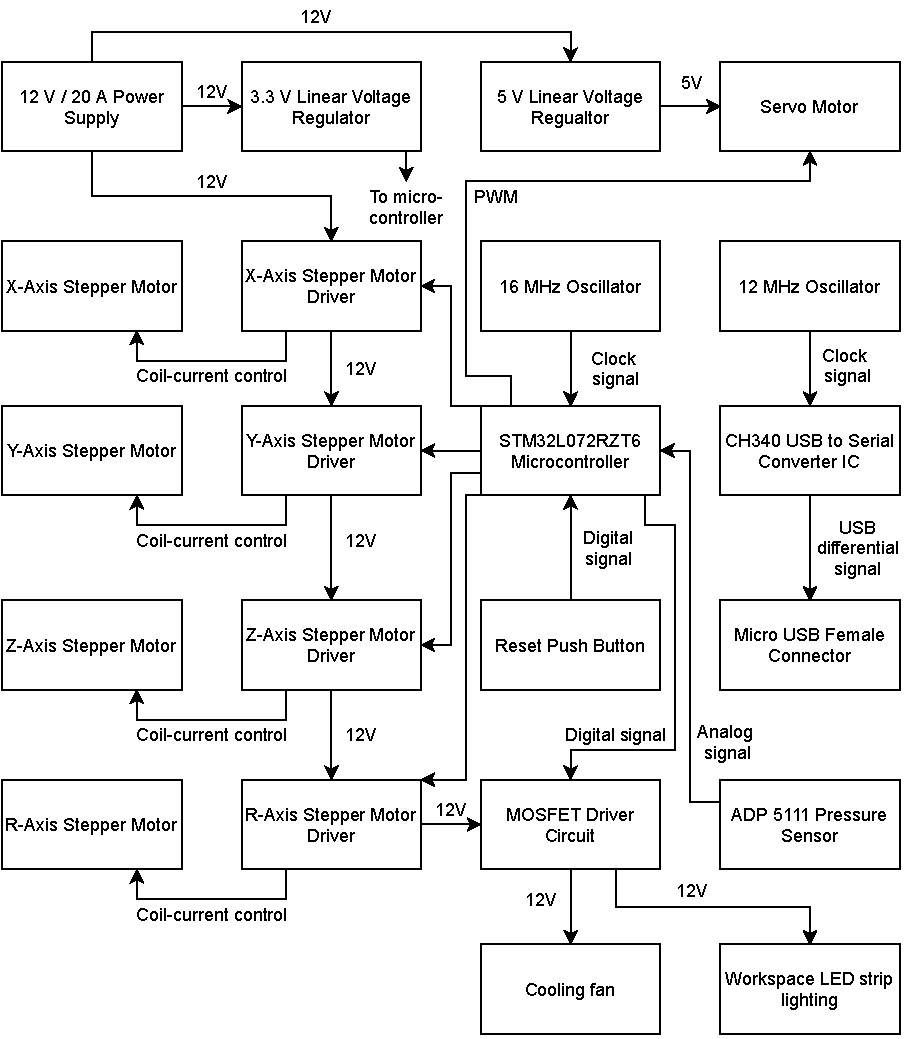
\includegraphics[scale=1]{figures/system-diagram.pdf}
	\caption{System block diagram of the hardware component of the system.}
	\label{fig:system-diagram}
\end{figure}

\newpage

\subsection{Record 2.  Systems level description of the design}

The hardware component of the system that is captured by the system block diagram shown in Figure \ref{fig:system-diagram} consists of three primary components. The first component is the hardware that forms part of the embedded robotic controller itself. The second is the servo motor and pressure sensor that form part of the vacuum generation mechanism while the third is the set of stepper motors used to drive the robotic manipulator. The entire hardware component is centred around the STM32L072RZT6 microcontroller. In order to power the system, a 12 V  and 20 A power supply was used. Since components operate at different voltage levels within the system, there is also a 3.3 V and a 5 V linear voltage regulator. The microcontroller itself uses the 3.3 V linear voltage regulator and is clocked by a 16 MHz oscillator. The microcontroller controls each of the robotic manipulator stepper motors through the use of DRV8825 stepper motor drivers. These take a 3.3 V signal as input and pass the 12 V power through to the stepper motors in a controlled fashion. The vacuum system servo motor is powered by the 5 V linear regulator and controlled by the microcontroller with a 3.3 V PWM signal. Similarly, the microcontroller also uses MOSFET circuits to control a cooling fan and the system workspace lighting. Lastly, the microcontroller takes an analog signal from the vacuum system pressure sensor as input to an ADC.

\newpage

\subsection{Record 3. Complete circuit diagrams and description}

See the next three pages for complete schematic of the embedded robotic subsystem controller circuit schematic that was created as part of the PCB design process.

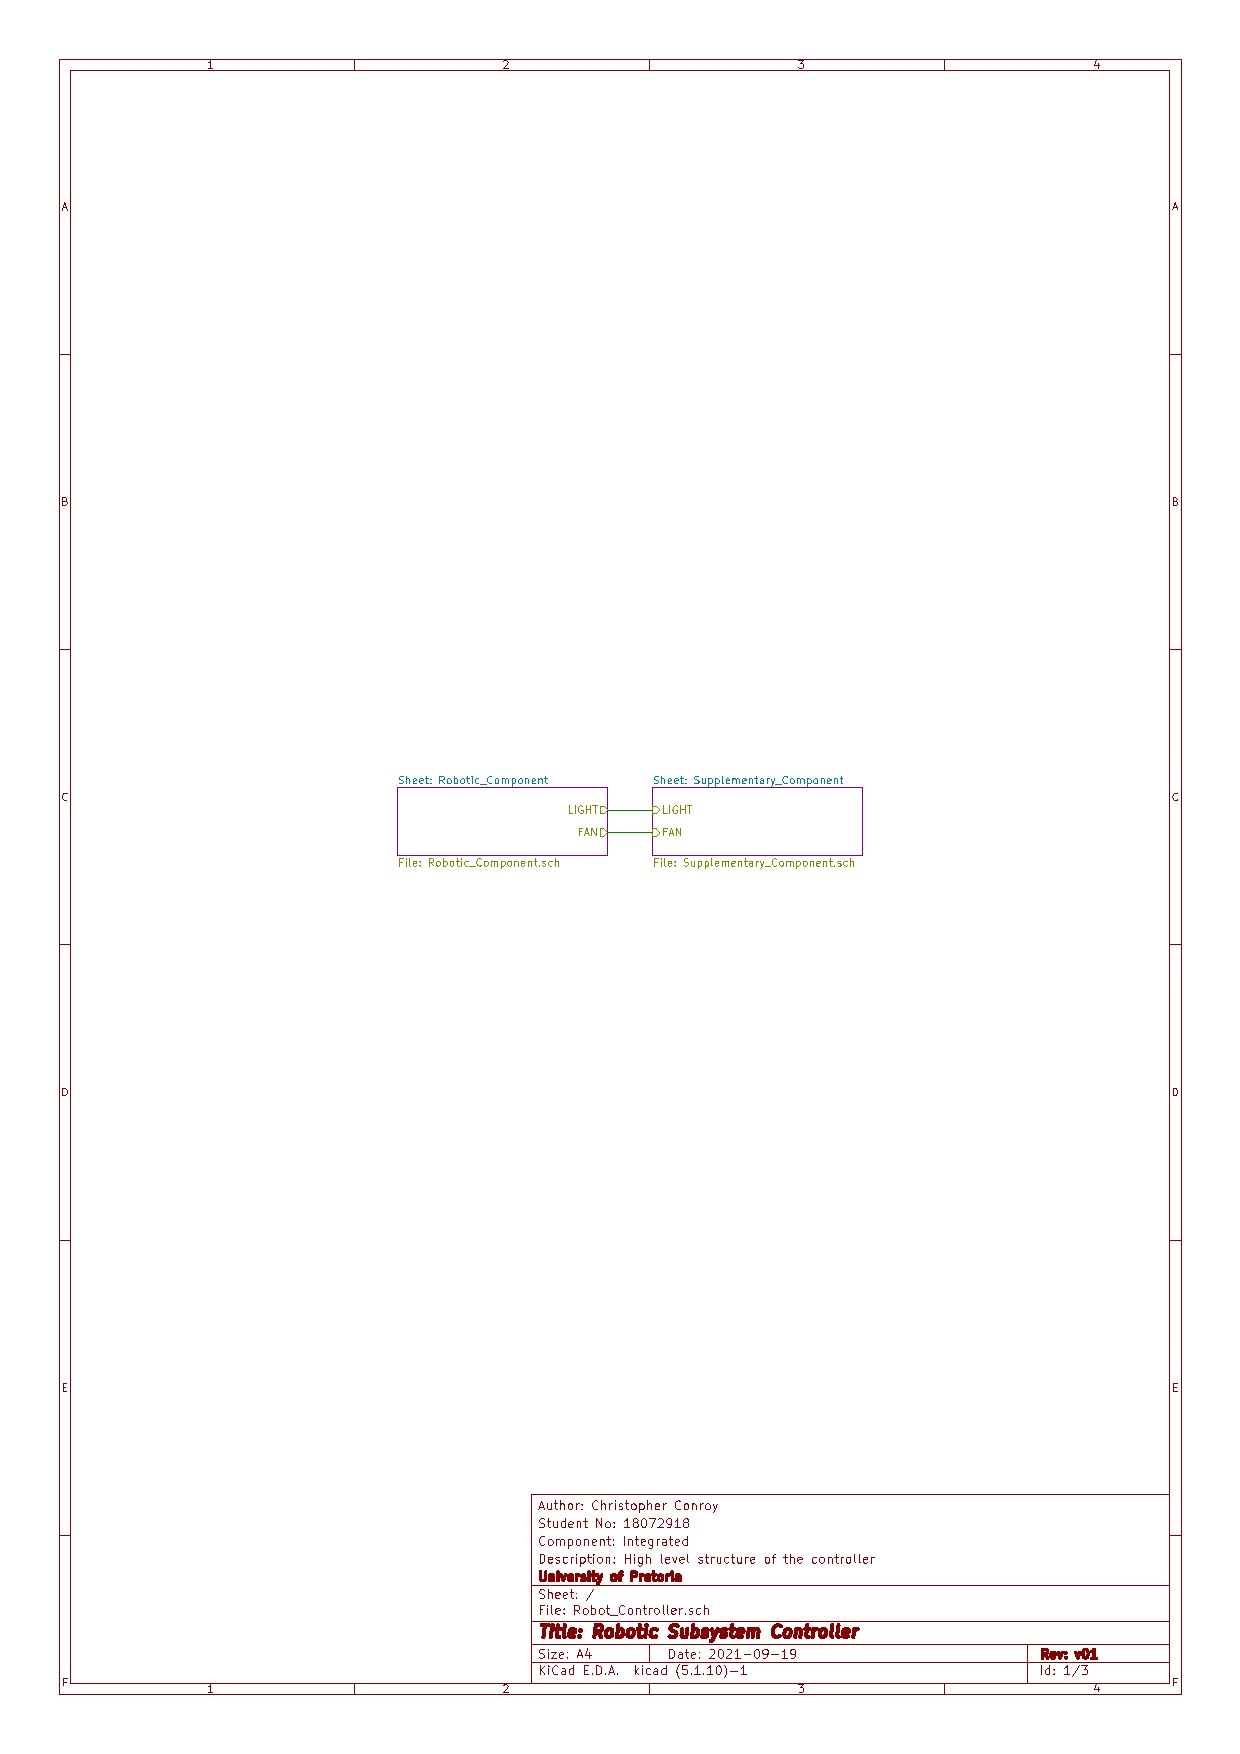
\includepdf[pages=-]{pdfs/electrical-design.pdf}

\subsection{Record 4. Hardware acceptance test procedure}

The functionality of the hardware can be verified using the following procedure:

\begin{compactenum}
	\item Connect the power supply to main's electricity using the three point plug.
	\item Verify that the green light power light on the PCB turns on to indicate that the hardware is receiving power.
	\item Connect the micro USB port on the embedded controller to the USB A port on a PC.
	\item Send a pressure sensor request packet to the hardware as detailed in the serial communication design section.
	\item Verify the receive and transmit lights both flash to indicate the hardware is responsive.
\end{compactenum}


\newpage

\subsection{Record 5. User guide}

The hardware can be set up for use by performing the following steps:

\begin{compactenum}
	\item Ensure that all the stepper motor cables, servo motor cable, pressure sensor cable, lighting cable and cooling fan cable are connected to the marked connectors on the board.
	\item Connect the power supply to main's electricity using the three point plug.
	\item Verify that the green light power light on the PCB turns on to indicate that the hardware is receiving power.
	\item Connect the micro USB port on the embedded controller to the USB A port on a PC.
	\item Start the system control software.
	\item Select the robot's serial port and connect the embedded controller using the \textit{Connect} button.
	\item If a connection is successfully established, the system is ready to use.
\end{compactenum}

\newpage

%% --------------------------------------------------------------------

\section{SOFTWARE part of the project}

\subsection{Record 6. Software process flow diagrams}

\begin{figure}[!ht]
	\centering
	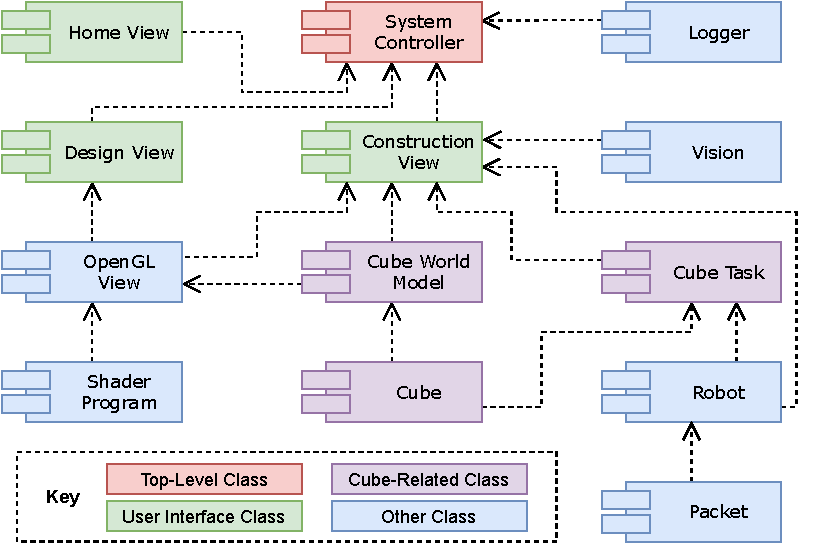
\includegraphics[scale=1]{figures/component-diagram.pdf}
	\caption{Component diagram showing the structure of the integrated PC-based software solution.}
	\label{fig:component-diagram-techdoc}
\end{figure}

\newpage

\subsection{Record 7. Explanation of software modules}

The \textit{System Controller} class shown in Figure \ref{fig:component-diagram-techdoc} sits at the top level of this implementation and directly contains the user interface classes\footnote{Each of the user interface classes correspond to a distinct screen in the user interface.} as well as the \textit{Logger} class through which all system event information, warnings and errors are recorded. The user interface classes partition the software based on functionality requirements. Specifically, the \textit{Home View} serves as the entrance point to the software and its purpose is to ensure the \textit{Robotic System} and camera hardware are present and connected. The \textit{Design View} integrates the components related to the \textit{Shape Definition} function. This includes the \textit{OpenGL View} which uses OpenGL to create a 3D render of a model of cubes. This class is supported by the \textit{Shader Program} class which manages the shaders used for the rendering task. The model itself is sourced from the \textit{Cube World Model} class. The purpose of this class is to simply capture the arrangement of cubes, which are each represented by an instance of the \textit{Cube} class, and relate this arrangement to the world coordinate system. The \textit{Design View} interface facilitates the creation and manipulation of a \textit{Cube World Model} instance which serves as output from the \textit{Shape Definition} component.

The \textit{Cube World Model} instance created in the \textit{Design View} acts as input to the construction process around which the \textit{Construction View} class is based. In order for construction to take place, the system needs to interact with the robot. The \textit{Robot} class was created for this purpose. The class provides an abstract interface for the \textit{Construction View} instance to send position and actuation control commands to the \textit{Robotic System}. The units of communication which the \textit{Robot} class uses to interact with embedded robotic controller are abstracted in the form of the \textit{Packet} class. This class is based on the packet designed in Section \ref{sec:Serial Communication}. Similarly, the \textit{Vision} class exists to offer an abstract interface to the \textit{Vision System} developed in Section \ref{sec:Computer Vision System}. The \textit{Construction View} instance receives information from this component that is used to guide the control of the \textit{Robot} instance during the construction process accordingly.

\newpage

\subsection{Record 8. Complete source code}
Complete code has been submitted separately on the AMS.

\newpage

\subsection{Record 9. Software acceptance test procedure}

In order to make use of the PC-based software's full functionality, a connection to the \textit{Robotic System} is required. Therefore, the the user guide for the hardware setup should first be followed. After completing this process, the software should have an established connection with the \textit{Robotic System}. Following this, navigate tot the \textit{Construction} view in the software. On this screen, click the \textit{Calibrate} button. The robot calibration sequence should be begin and carry out to completion successfully. This verifies that the software is functioning correctly.

\newpage

\subsection{Record 10. Software user guide}

This section assumes that the software has been verified to be functioning correctly with the software acceptance test procedure. The system control software is started by running the PC-based software executable file. The initial screen displayed is the home screen as shown in Figure \ref{fig:gui-home}. A feed from the camera of the robot's workspace should be displayed to indicate the camera's presence. The system message log for informational messages, warnings and errors is displayed at the bottom of the screen. The messages can be filtered as needed with the filter checkboxes. Connect to the robot by selecting the CH340 serial port from the serial port list and clicking the \textit{Connect} button.

The \textit{Shape Definition} component can be accessed by clicking on the \textit{Shape Design} button. This screen is shown in Figure \ref{fig:gui-design-view}. The set of buttons in the top left can be used to insert and remove cubes from the build as well as to load and save model designs. Individual cubes can be selected in the left cubes list. Use the arrow keys to translate the cube horizontally. Use the shift button with the arrow keys to move the cube vertically and to rotate the cube. Use the mouse buttons to move the camera around the structure.

The \textit{Construction} view can be accessed by clicking on the \textit{Construction} button. This view is shown in Figure \ref{fig:gui-construction-view}. The first group of buttons can be used to calibrate the robot, apply the computer vision system to the current scene, load a model for construction and start a construction sequence. The vision view and model views shown in Figures \ref{fig:gui-vision-view} and \ref{fig:gui-vision-view-model} respectively. The next set of buttons are used to set the active state of the stepper motors and control the vacuum actuator state. Finally the last set of controls allows the control of the position of the robot.

The vision view shown in Figure \ref{fig:gui-vision-view} is used to set the annotations and stage displayed for the image display. Examples of these stages are shown in Figures \ref{fig:gui-vision-view-contour} and \ref{fig:gui-vision-view-fiducial}. Finally, the model view in Figure \ref{fig:gui-vision-view-model} can be used to select the 3D render displayed. Either the shape to be built is displayed, or the live location of the cubes during construction is displayed.

\begin{figure}[!ht]
	\centering
	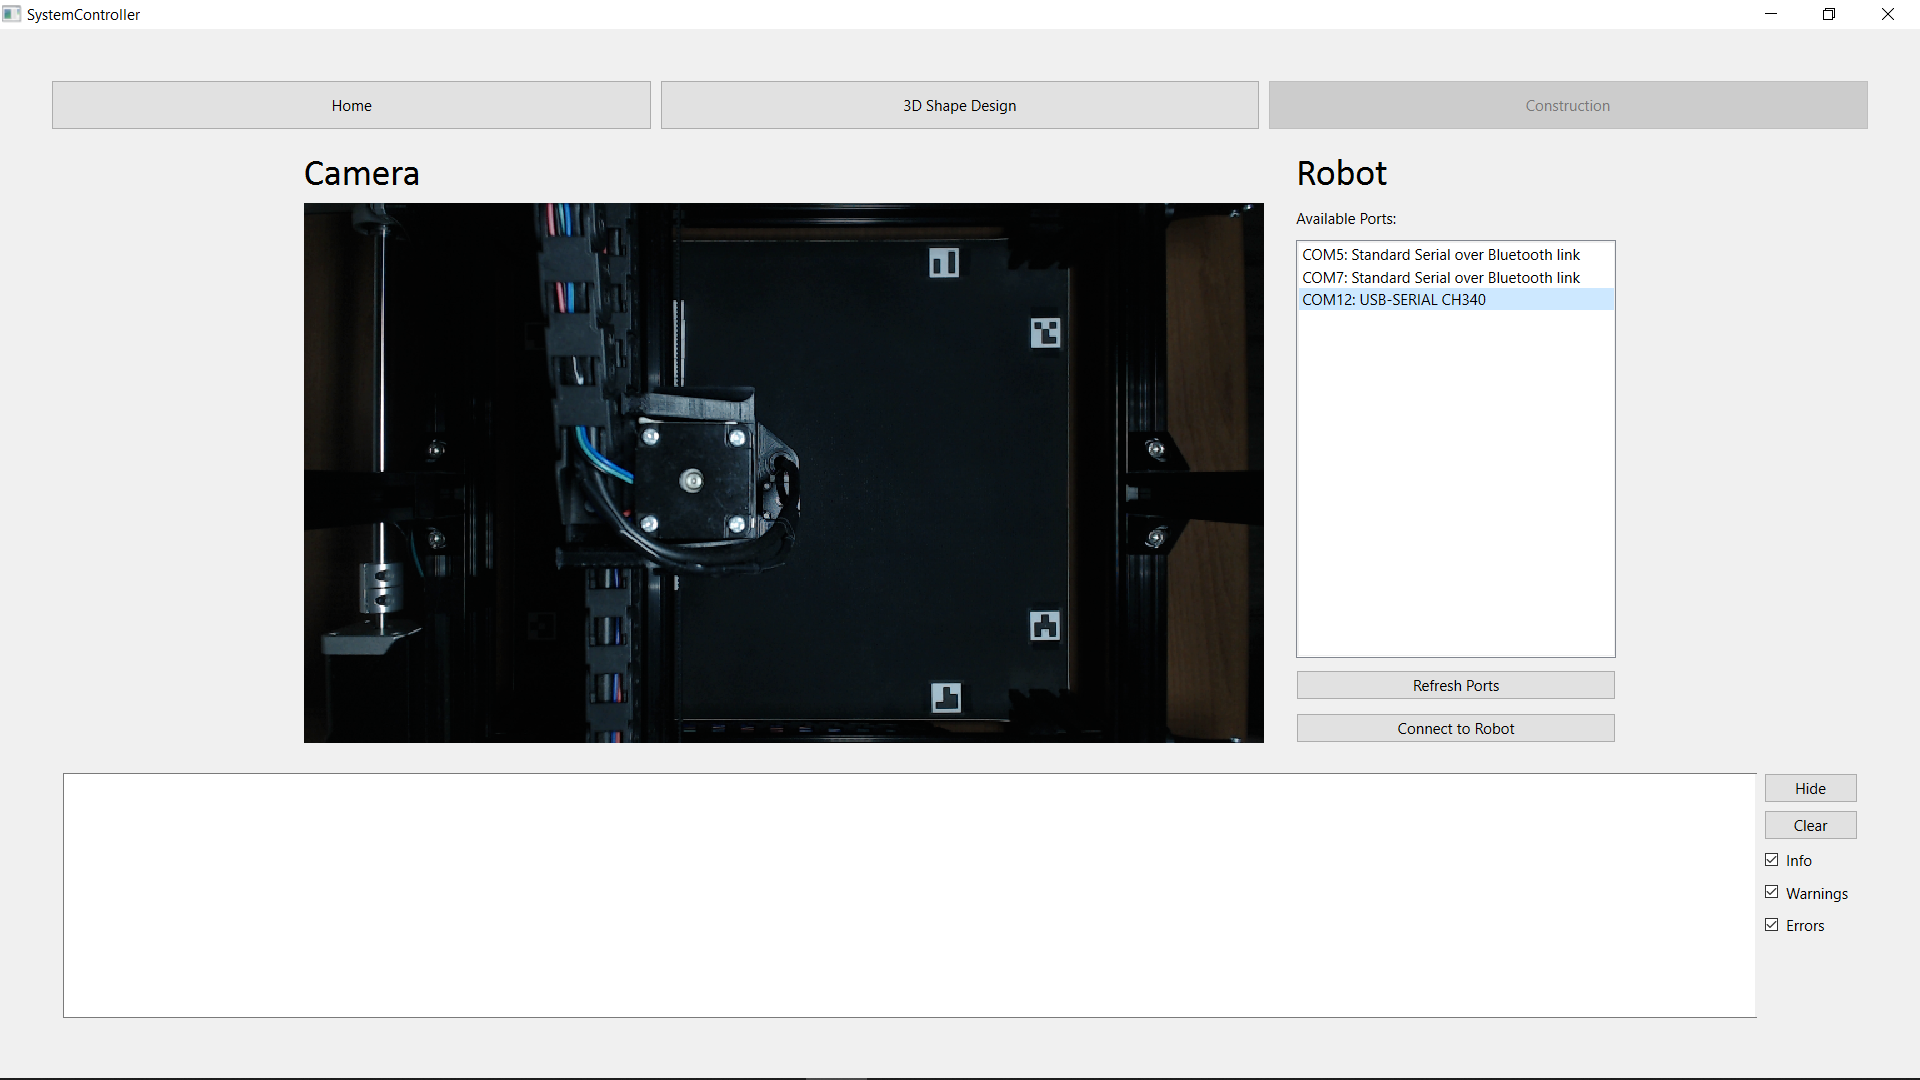
\includegraphics[width=1\linewidth]{figures/gui-home.png}
	\caption{System control software home screen.}
	\label{fig:gui-home}
\end{figure}

\begin{figure}[!ht]
	\centering
	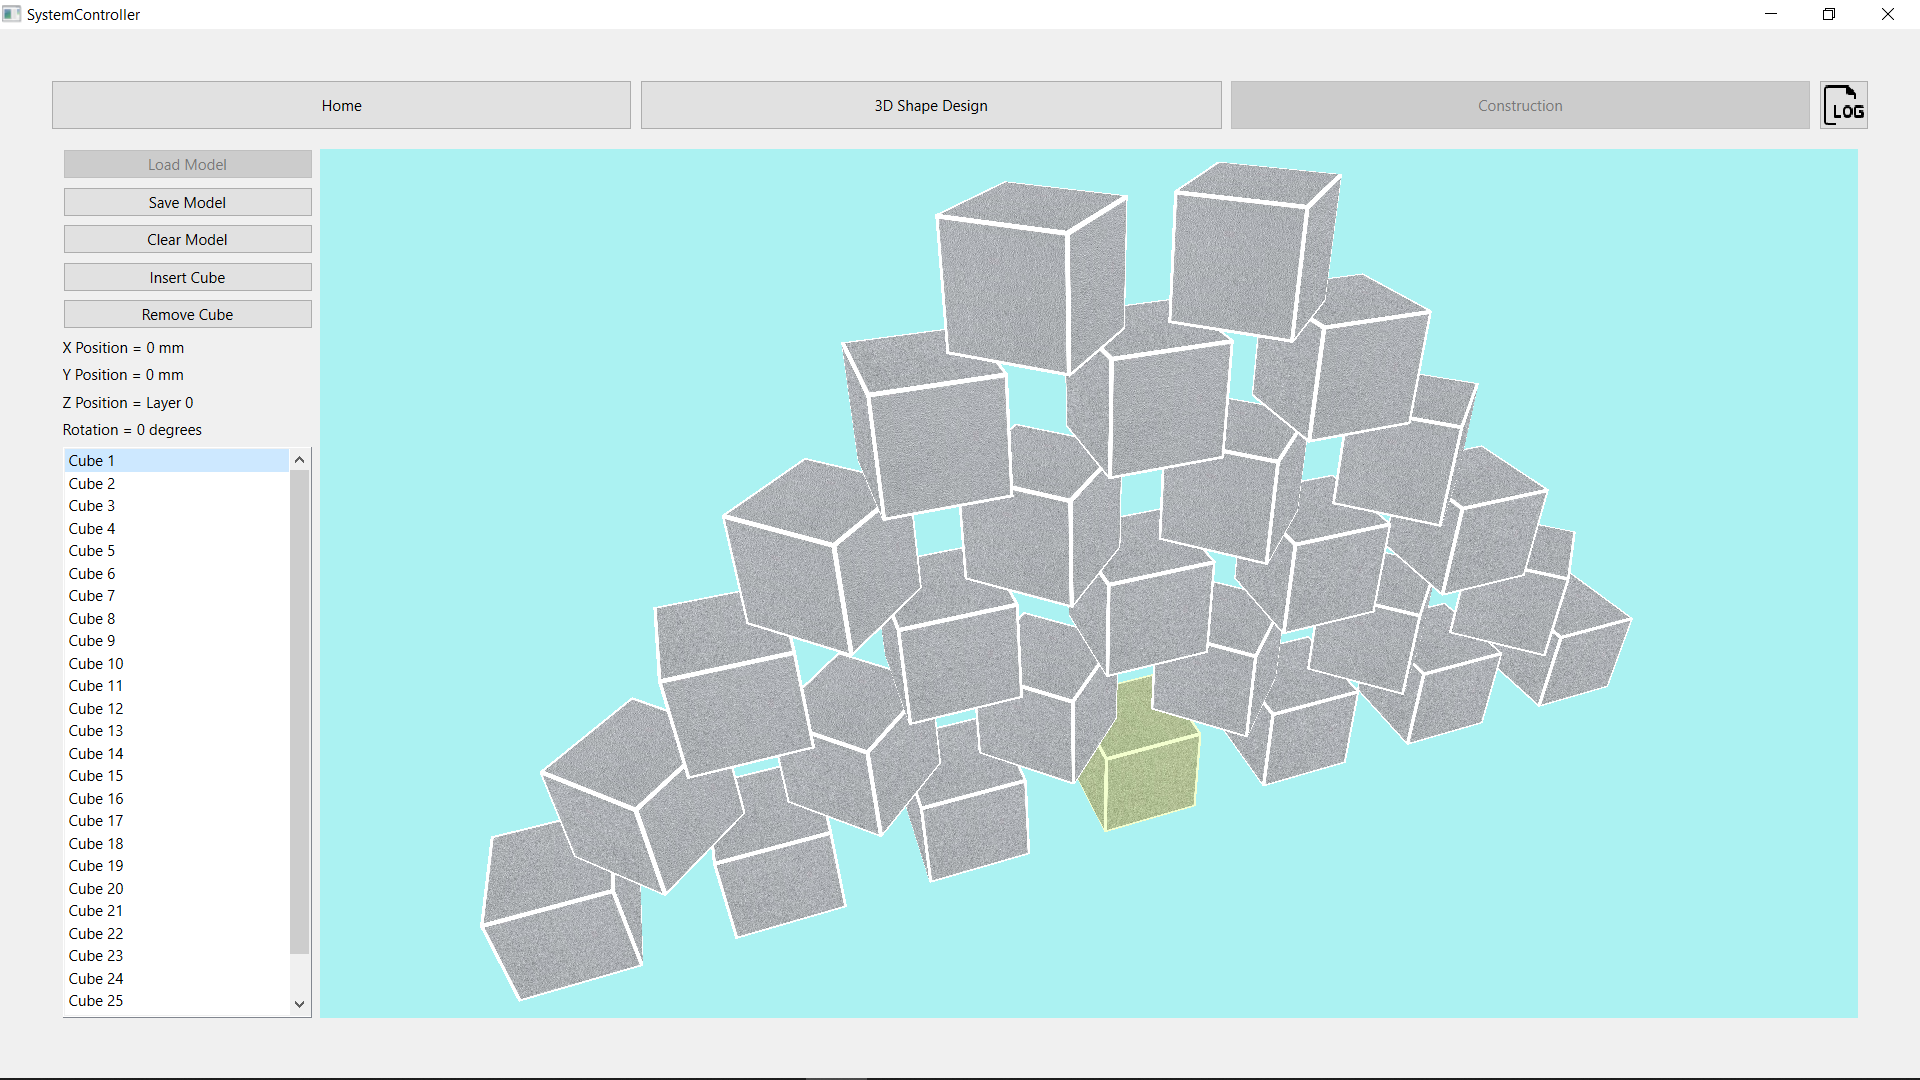
\includegraphics[width=1\linewidth]{figures/gui-design-view.png}
	\caption{System control software 3D shape design screen.}
	\label{fig:gui-design-view}
\end{figure}

\begin{figure}[!ht]
	\centering
	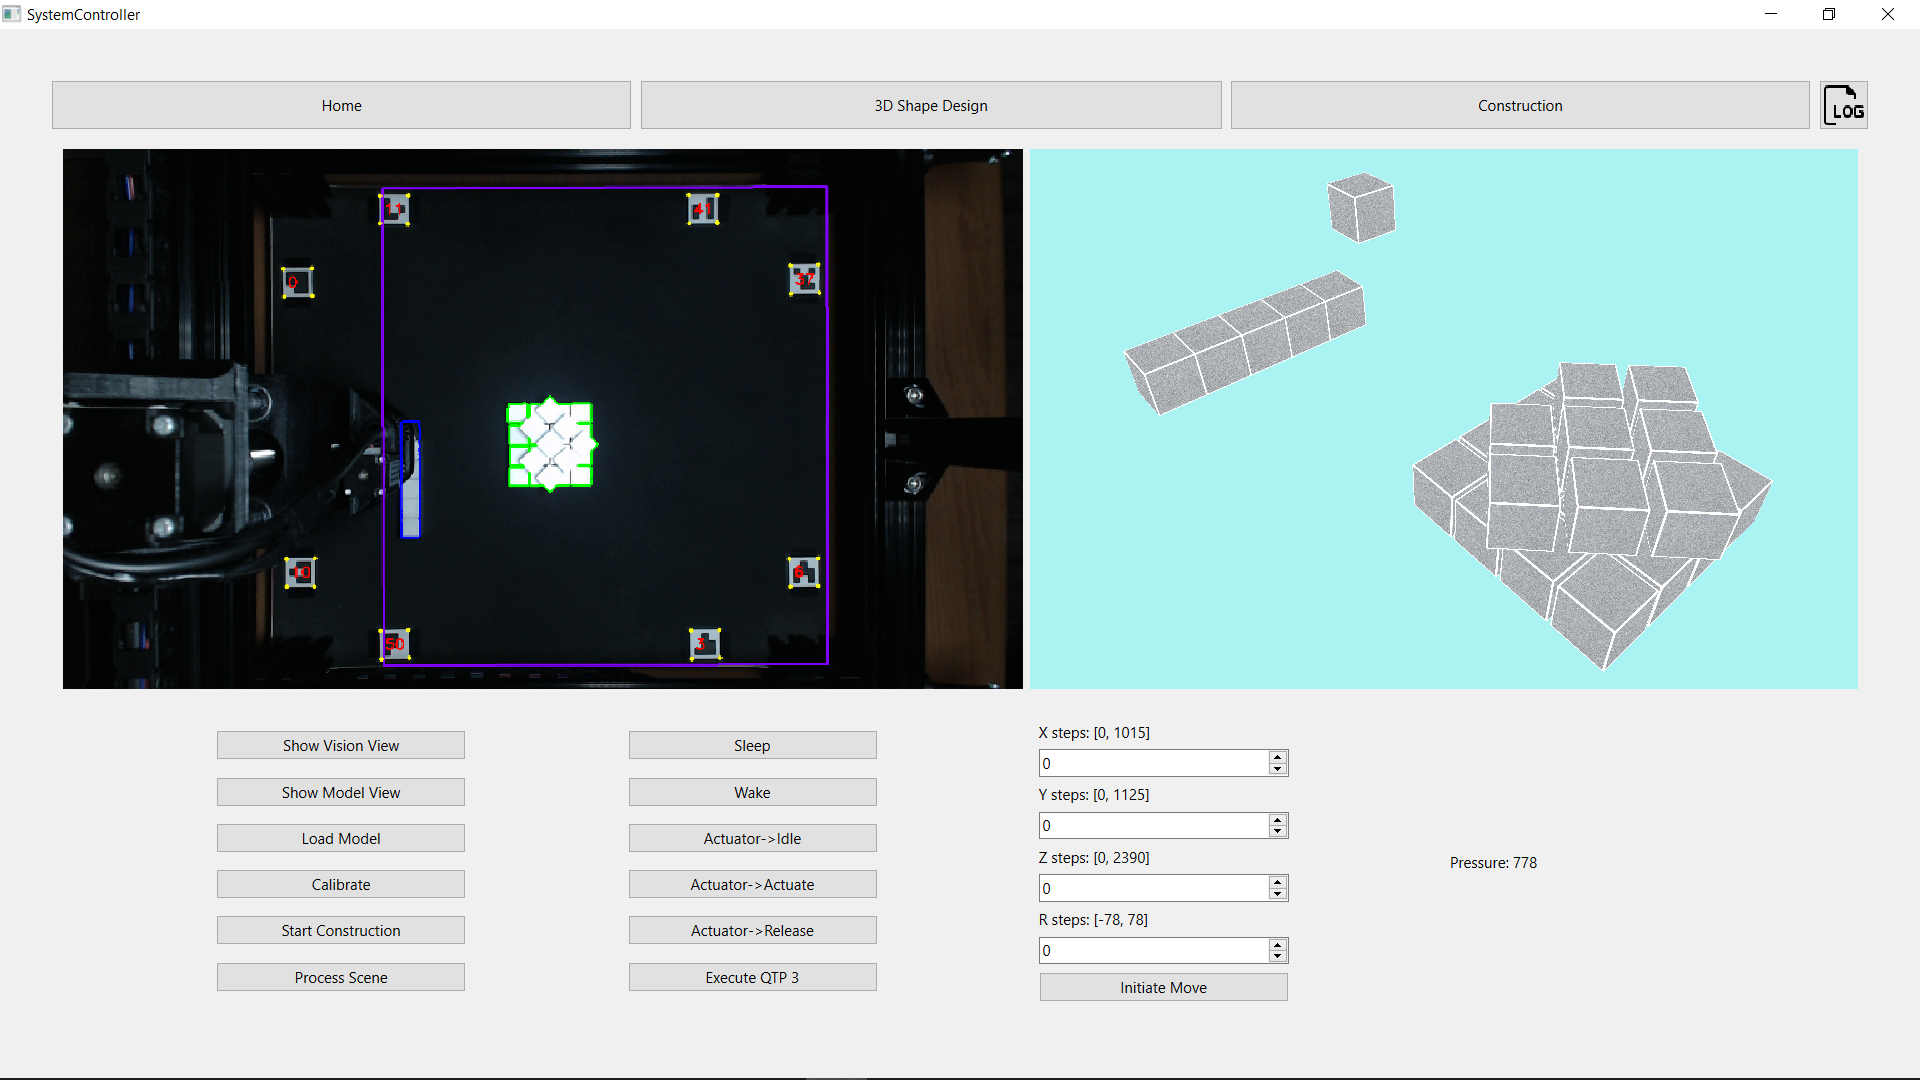
\includegraphics[width=1\linewidth]{figures/gui-construction-view2.png}
	\caption{System control software home screen.}
	\label{fig:gui-construction-view}
\end{figure}

\begin{figure}[!ht]
	\centering
	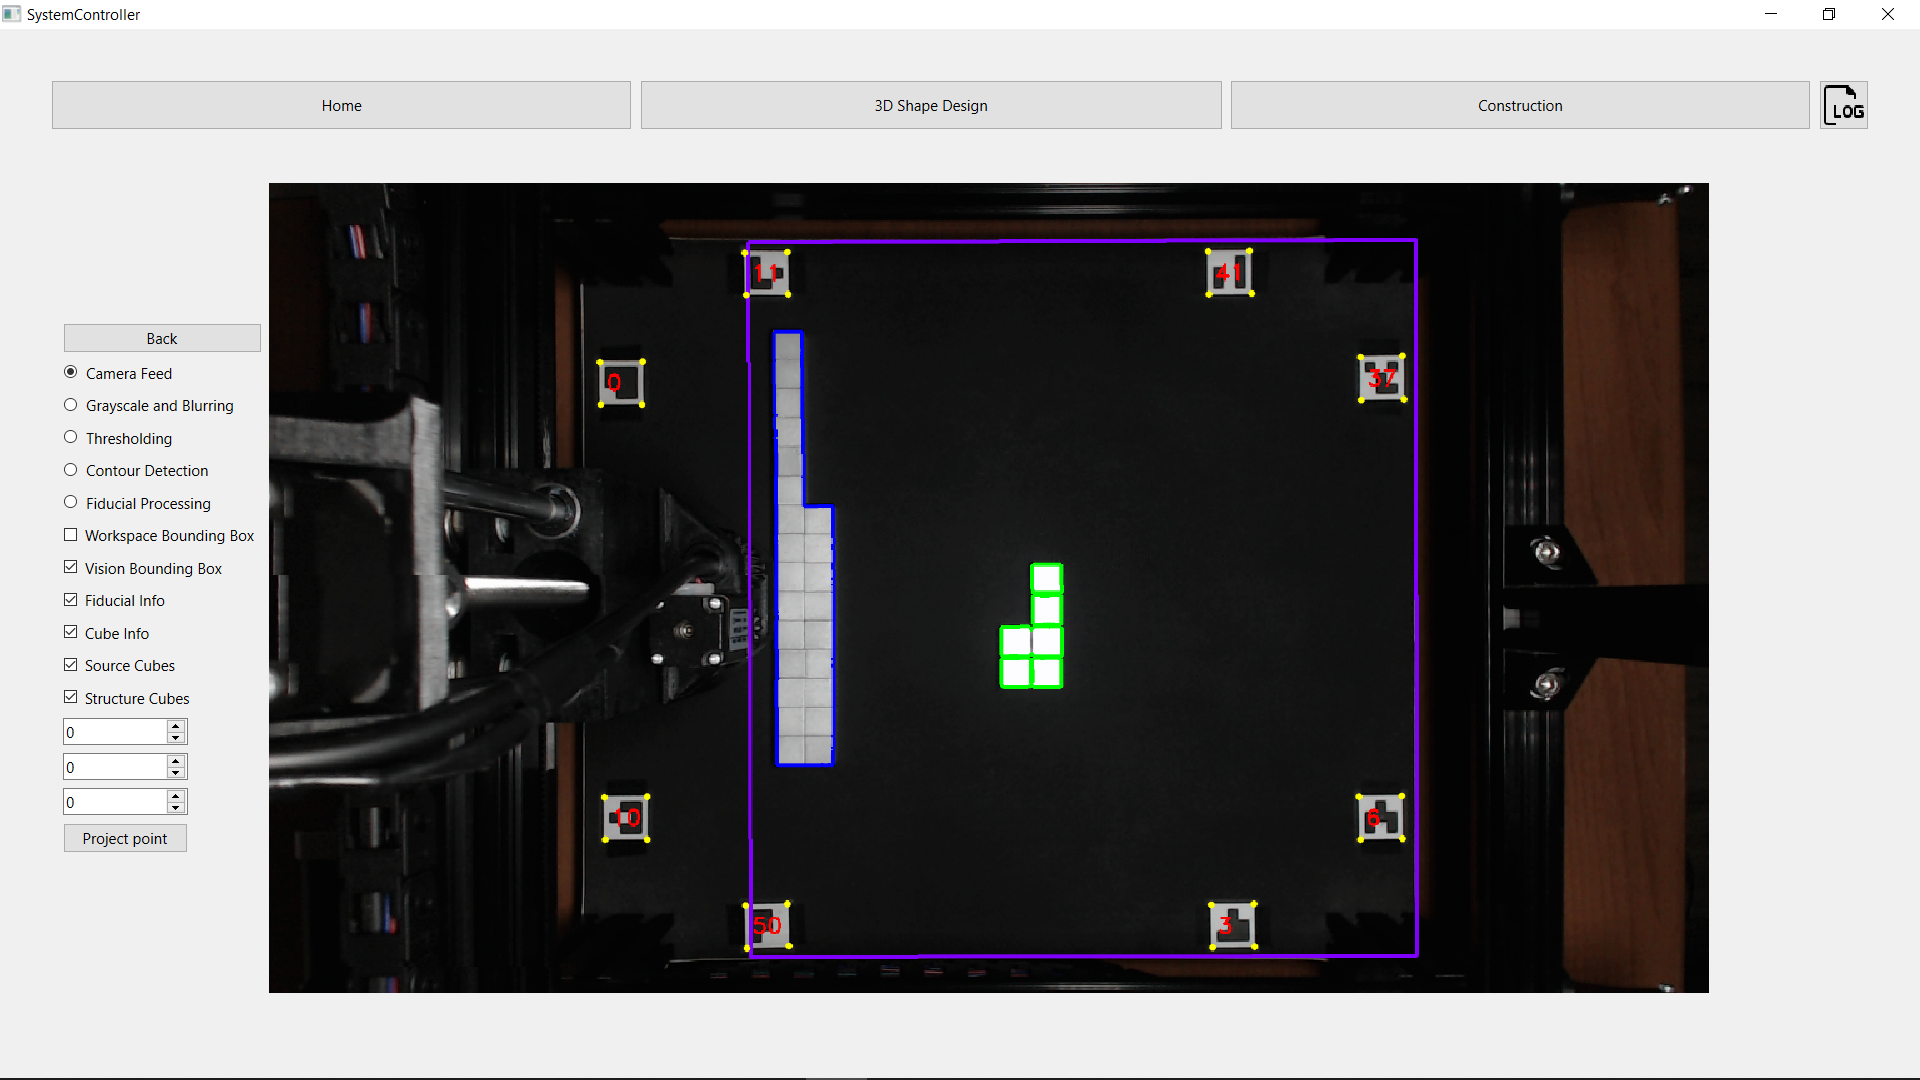
\includegraphics[width=1\linewidth]{figures/gui-vision-view.png}
	\caption{System control software home screen.}
	\label{fig:gui-vision-view}
\end{figure}

\begin{figure}[!ht]
	\centering
	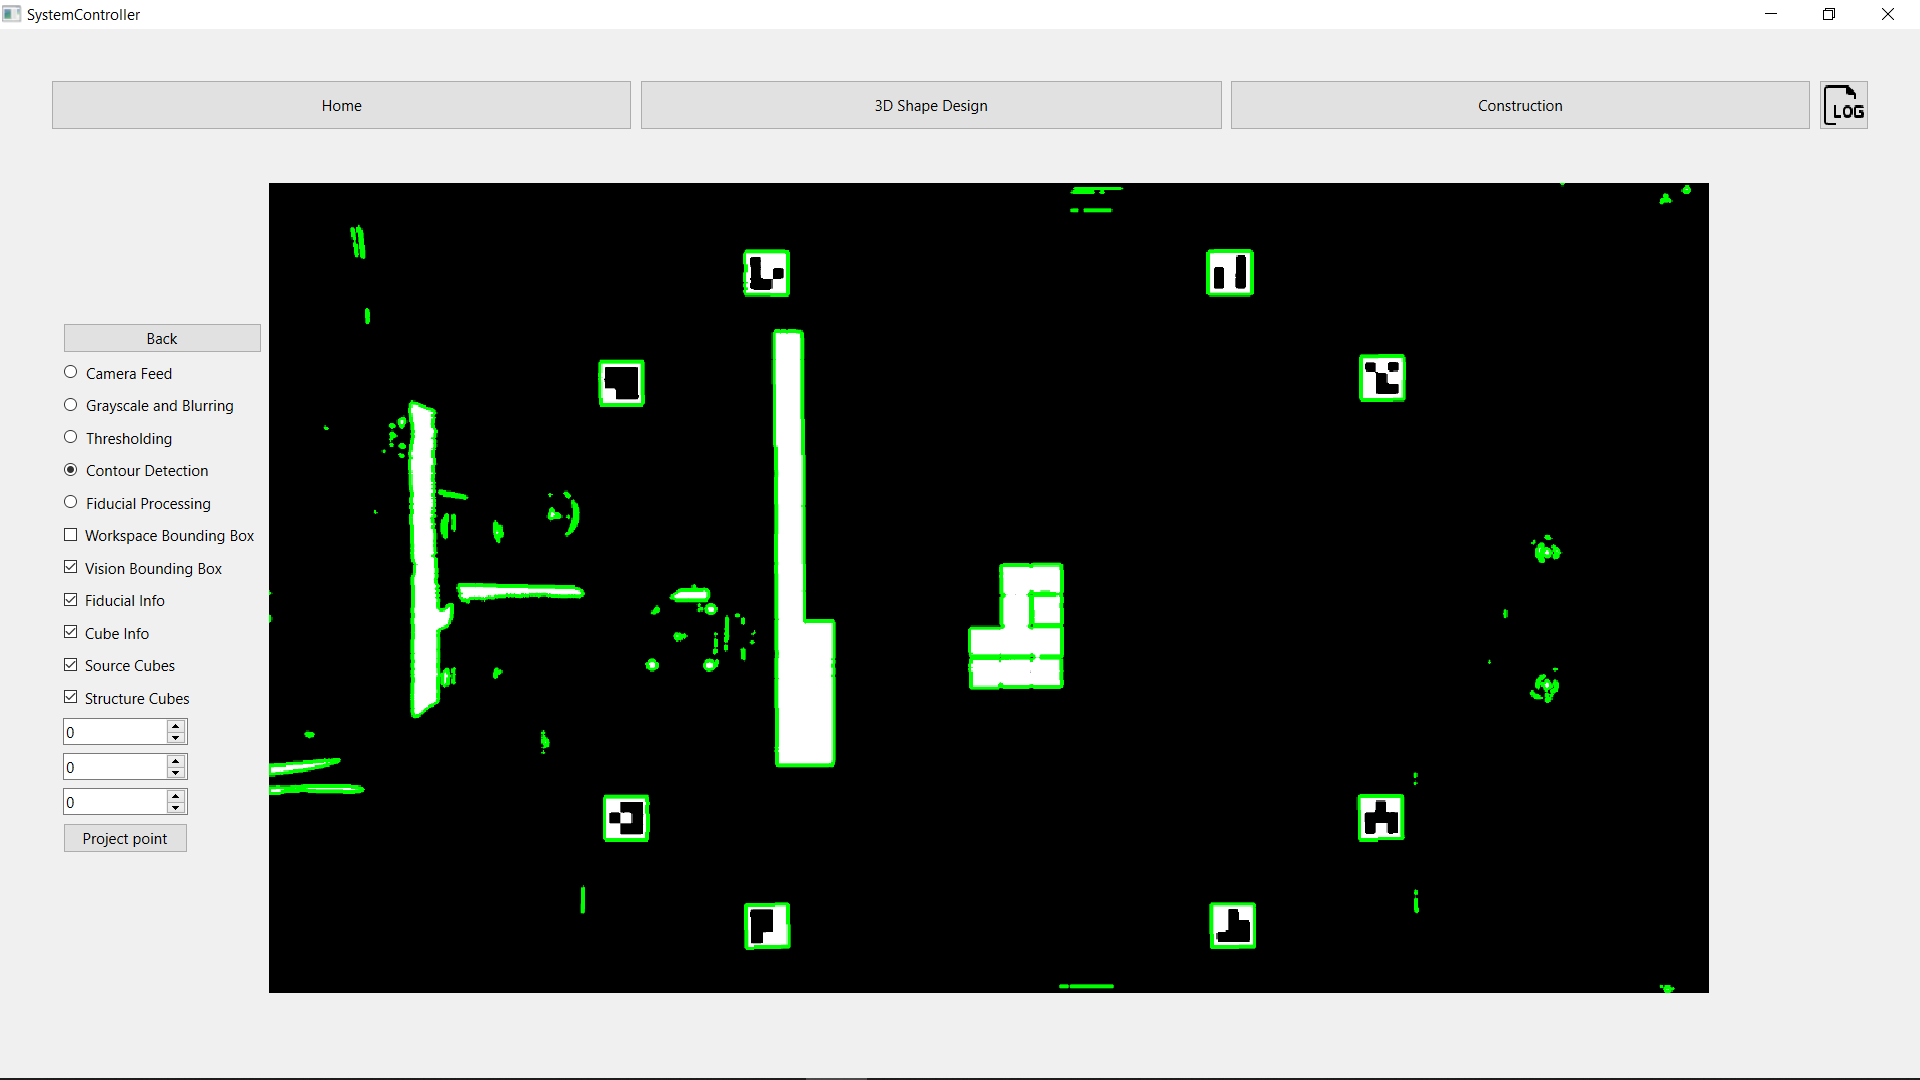
\includegraphics[width=1\linewidth]{figures/gui-vision-view-contour.png}
	\caption{System control software home screen.}
	\label{fig:gui-vision-view-contour}
\end{figure}

\begin{figure}[!ht]
	\centering
	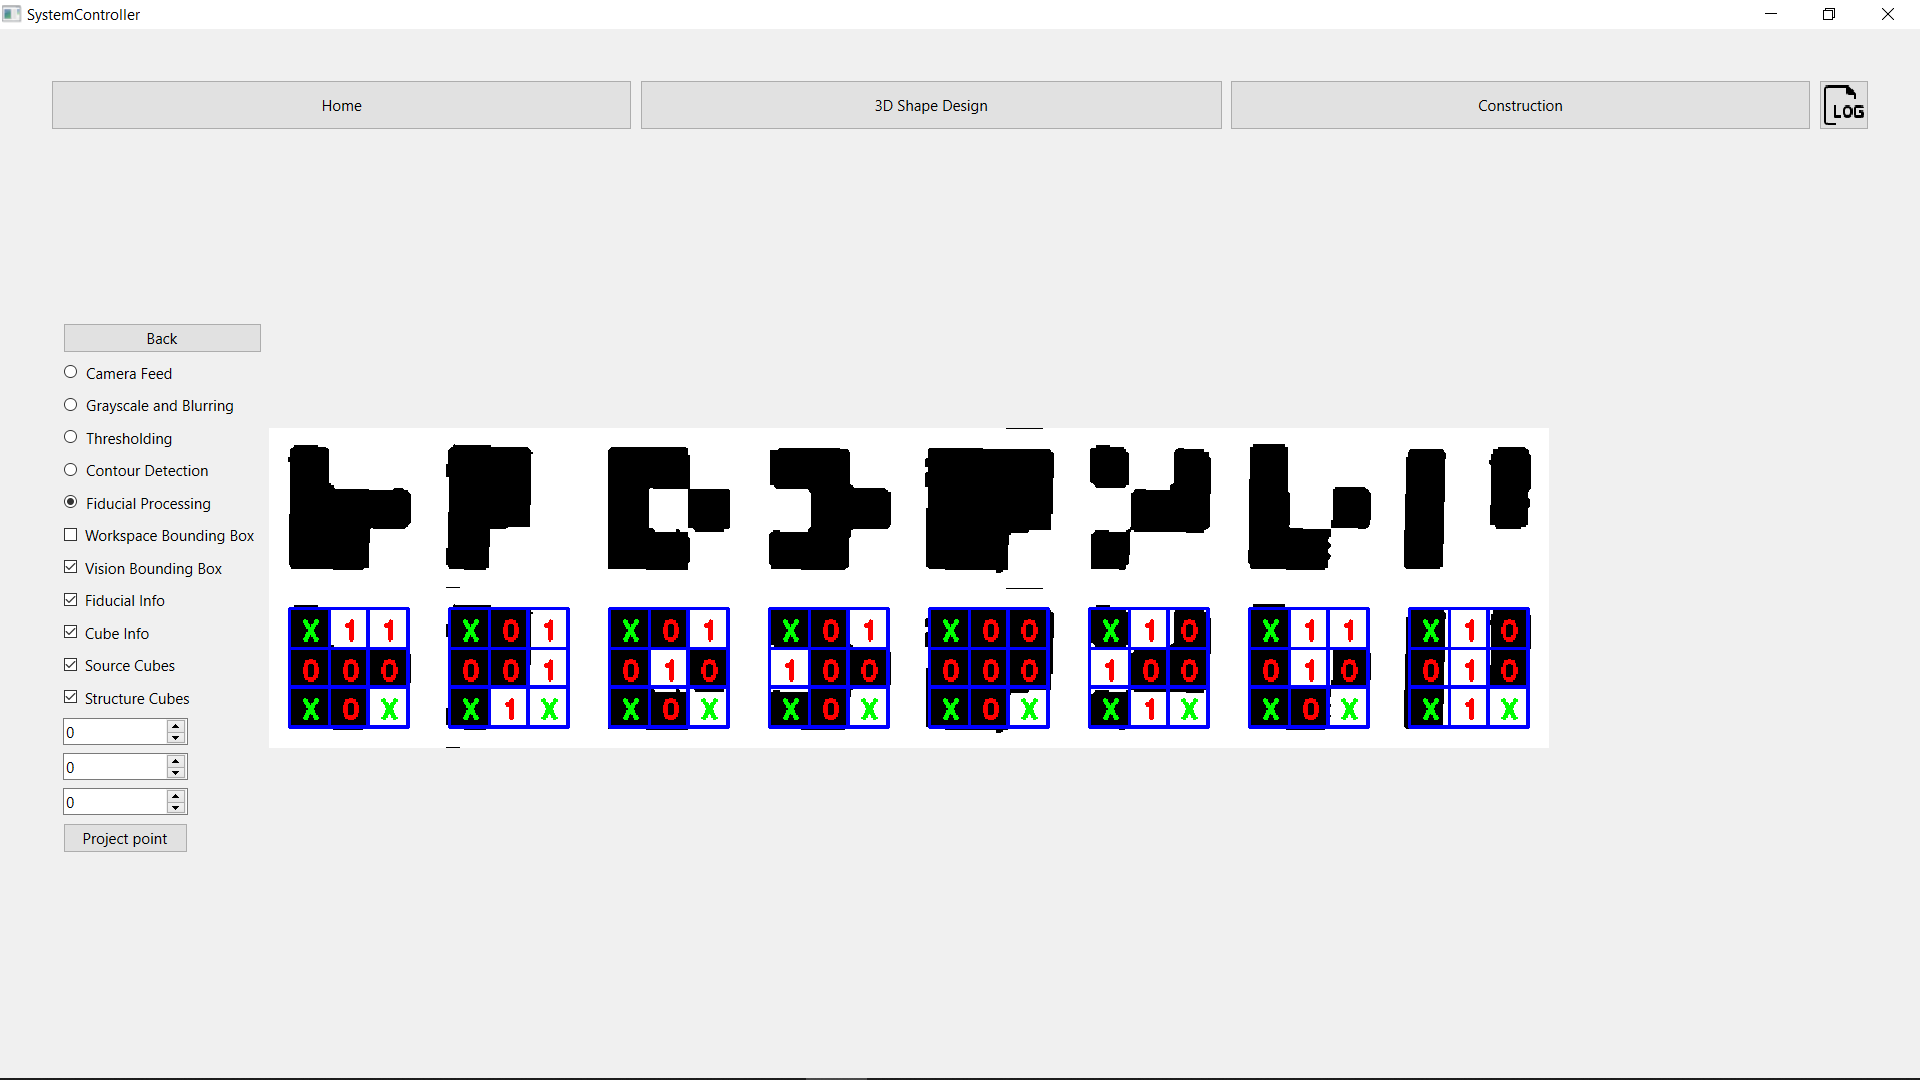
\includegraphics[width=1\linewidth]{figures/gui-vision-view-fiducial.png}
	\caption{System control software home screen.}
	\label{fig:gui-vision-view-fiducial}
\end{figure}

\begin{figure}[!ht]
	\centering
	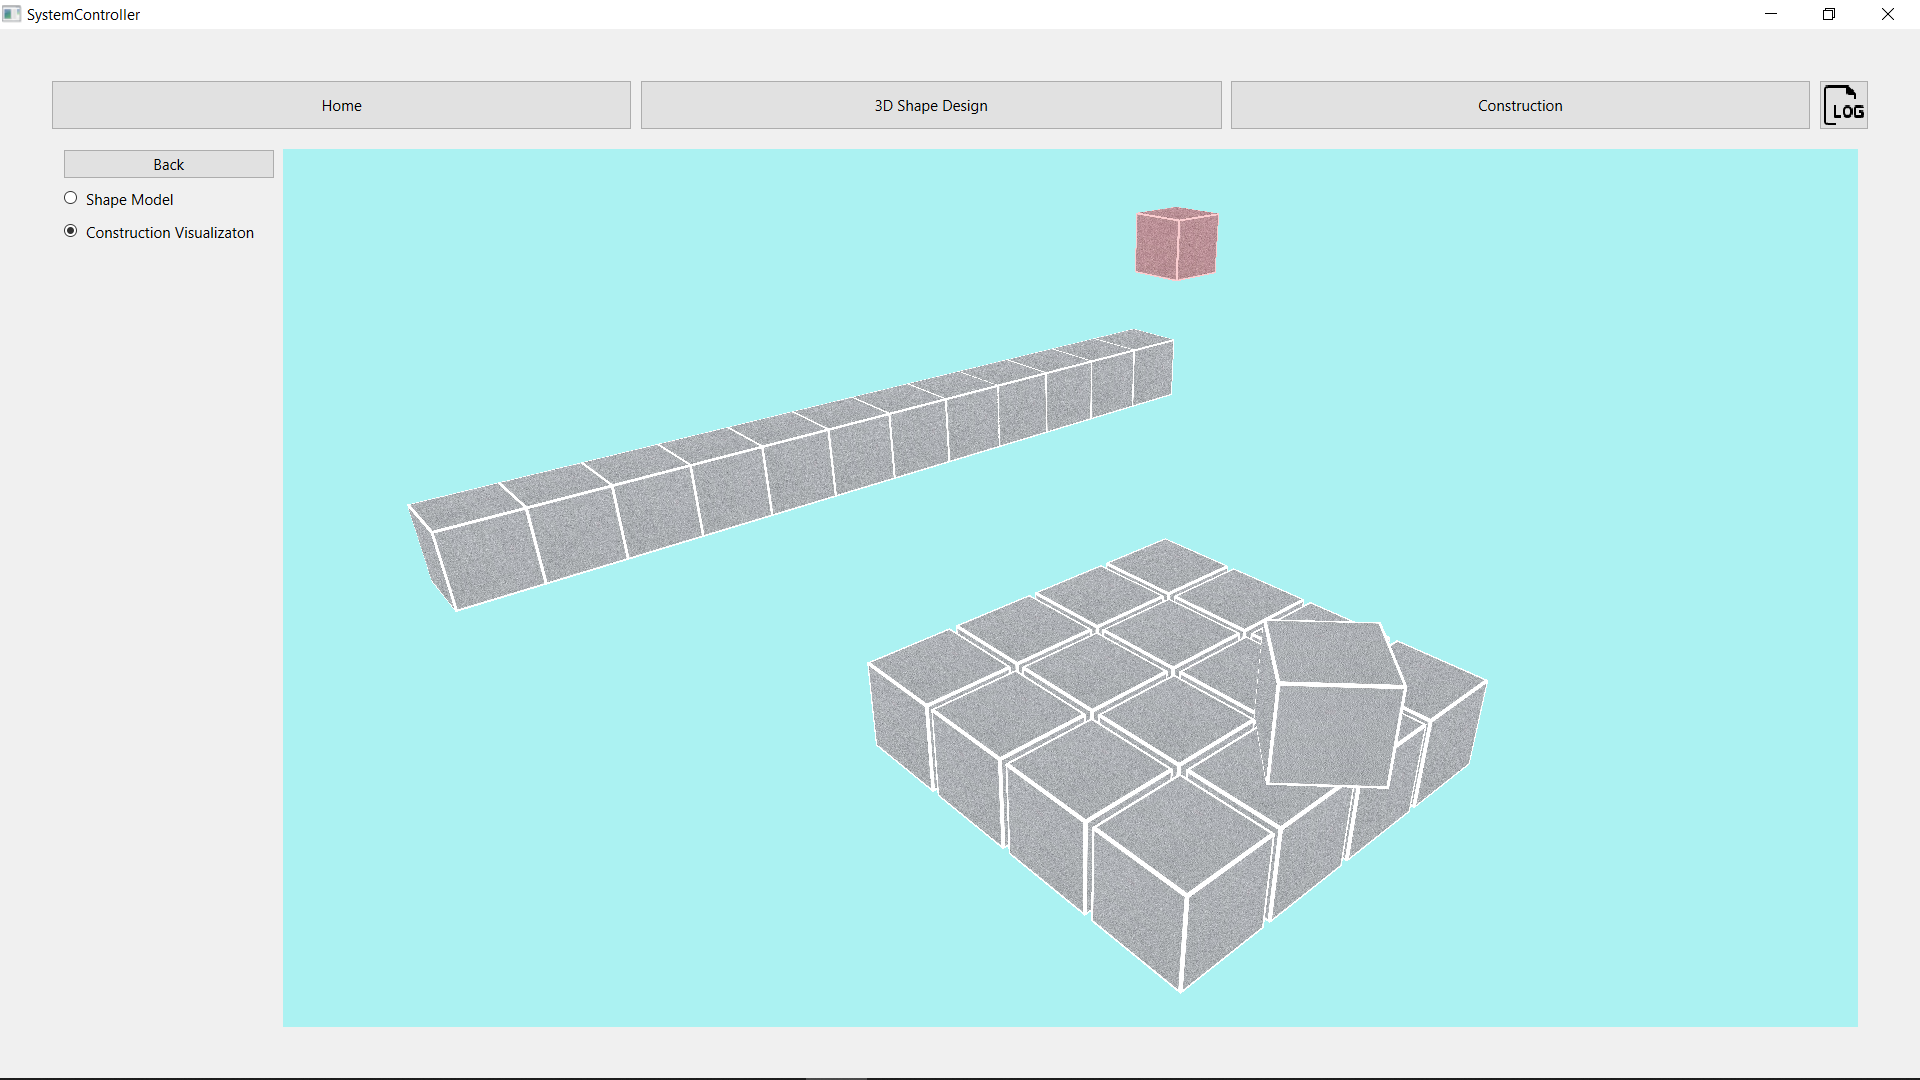
\includegraphics[width=1\linewidth]{figures/gui-model-view.png}
	\caption{System control software home screen.}
	\label{fig:gui-vision-view-model}
\end{figure}

\newpage

%% --------------------------------------------------------------------

\section{EXPERIMENTAL DATA}

\subsection{Record 11. Experimental data}

\subsubsecnonumhidden{Qualification Test 1 Results}

A test set of 10 3D shape models was defined using the \textit{Shape Definition} component for use in qualification test 1. Table \ref{tab:techdoc-qtp1-properties} summarises the important properties of each of these shapes

% Shape 1 - pyramid
% Shape 2 - Rotated pyramid
% Shape 3- Extended bridge
% Shape 4 - Sparse triangle
% Shape 5 - Stress test shape
% Shape 6 - 5 stacks of 6 cubes
% Shape 7- Bridge supporting rotated cubes
% Shape 8 - 
% Shape 9 - Bridge
% Shape 10 - Spread pyramid

\begin{table}[H]
	\renewcommand{\arraystretch}{1.3}
	\centering
	\begin{tabular}{|>{\raggedright}m{1.1cm}|>{\raggedright}m{2cm}|>{\raggedright}m{2cm}|>{\raggedright}m{2cm}|>{\raggedright}m{2cm}|>{\raggedright\arraybackslash}m{2cm}|}
		\hline
		\textbf{Shape ID} & \textbf{Number of Cubes} & \textbf{Rotated Cubes} & \textbf{Partially Supported Cubes\footnotemark} & \textbf{Slanted Cube Stack} & \textbf{Shape Height} \\
		\hline
		1 & 30 & No & No & No & 4  \\ \hline
		2 & 30 & Yes & No & No & 4  \\ \hline
		3 & 30 & No & Yes & Yes & 6  \\ \hline
		4 & 30 & Yes & No & No & 6  \\ \hline
		5 & 30 & Yes & Yes & No & 5  \\ \hline
		6 & 30 & No & No & No & 6  \\ \hline
		7 & 30 & Yes & Yes & Yes & 6  \\ \hline
		8 & 30 & Yes & Yes & No & 6  \\ \hline
		9 & 30 & No & No & Yes & 6  \\ \hline
		10 & 30 & No & Yes & No & 4  \\ \hline
	\end{tabular}
	\caption{\label{tab:techdoc-qtp1-properties}Properties of each 3D shape model in the test set for qualification test 1.}
\end{table}

\footnotetext{A cube is considered to be partially supported if less than half of the bottom face of the cube is touching the top faces of the cubes in the layer below it.}

\begin{table}[H]
	\renewcommand{\arraystretch}{1.3}
	\centering
	\begin{tabular}{|>{\raggedright}m{2cm}|>{\raggedright}m{2cm}|>{\raggedright}m{2cm}|>{\raggedright}m{2cm}|>{\raggedright}m{2cm}|>{\raggedright\arraybackslash}m{2cm}|}
		\hline
		\textbf{Shape ID} & \textbf{Back Left} & \textbf{Back Right} & \textbf{Centre} & \textbf{Front Left} & \textbf{Front Right} \\
		\hline
		1 & Success & Success & Success & Success & Success  \\ \hline
		2 & Success & Success & Success & Success & Success  \\ \hline
		3 & Success & Success & Success & Success & Success  \\ \hline
		4 & Success & Success & Success & Success & Success  \\ \hline
		5 & Success & Success & Success & Success & Success  \\ \hline
		6 & Success & Success & Success & Success & Success  \\ \hline
		7 & Success & Success & Success & Success & Success  \\ \hline
		8 & Success & Success & Success & Success & Success  \\ \hline
		9 & Success & Success & Success & Success & Success  \\ \hline
		10 & Success & Success & Success & Success & Success  \\ \hline
	\end{tabular}
	\caption{\label{tab:techdoc-qtp1-results}Results of each shape construction sequence at 5 different locations in the robot's workspace.}
\end{table}

\subsubsecnonumhidden{Qualification Test 3 Results}

\begin{table}[H]
	\renewcommand{\arraystretch}{1.3}
	\centering
	\begin{tabular}{|>{\raggedright}m{1.6cm}|>{\raggedright}m{2.6cm}|>{\raggedright}m{3.2cm}|>{\raggedright}m{3.3cm}|>{\raggedright\arraybackslash}m{2.6cm}|}
		\hline
		\textbf{Iteration} & \textbf{Cube Gripped (Y/N)?} & \textbf{Time Dropped (s)} & \textbf{Move Sequence Completed (Y/N)?} & \textbf{Cube Released (Y/N)?} \\
		\hline
		1 & Yes & Not Dropped & Yes & Yes \\ \hline
		2 & Yes & Not Dropped & Yes & Yes \\ \hline
		3 & Yes & Not Dropped & Yes & Yes \\ \hline
		4 & Yes & Not Dropped & Yes & Yes \\ \hline
		5 & Yes & Not Dropped & Yes & Yes \\ \hline
		6 & Yes & Not Dropped & Yes & Yes \\ \hline
		7 & Yes & Not Dropped & Yes & Yes \\ \hline
		8 & Yes & Not Dropped & Yes & Yes \\ \hline
		9 & Yes & Not Dropped & Yes & Yes \\ \hline
		10 & Yes & Not Dropped & Yes & Yes \\ \hline
	\end{tabular}
	\caption{\label{tab:techdoc-qtp3}Results of the movement sequence iterations for qualification test 3.}
\end{table}

\subsubsecnonumhidden{Qualification Test 4 Results}

\begin{table}[H]
	\renewcommand{\arraystretch}{1.3}
	\centering
	\begin{tabular}{|>{\raggedright}m{1.5cm}|>{\raggedright}m{1.9cm}|>{\raggedright}m{1.9cm}|>{\raggedright}m{1.9cm}|>{\raggedright}m{1.8cm}|>{\raggedright}m{1.6cm}|>{\raggedright\arraybackslash}m{1.6cm}|}
		\hline
		\textbf{Sample Set} & \textbf{X Position (steps)} & \textbf{Y Position (steps)} & \textbf{Z Position (steps)} & \textbf{Reference Length (pixels)} & \textbf{X Points Range (pixels)} & \textbf{Y Points Range (pixels)} \\
		\hline
		1 & 0    & 0    & 0 & 79,168 & 9,751  & 8,03   \\
		\hline
		2 & 0    & 1125 & 0 & 61,265 & 13,883 & 11,059 \\
		\hline
		3 & 507  & 562  & 0 & 70,112 & 15,882 & 12,176 \\
		\hline
		4 & 1015 & 0    & 0 & 75,279 & 15,853 & 12,257 \\
		\hline
		5 & 1015 & 1125 & 0 & 72,198 & 11,063 & 8,388 \\
		\hline
	\end{tabular}
	\caption{\label{tab:techdoc-qtp4-xy1}Pixel measurements using the point cluster images for the x- and y-axis repeatability test.}
\end{table}

\begin{table}[H]
	\renewcommand{\arraystretch}{1.3}
	\centering
	\begin{tabular}{|>{\raggedright}m{2.5cm}|>{\raggedright}m{4cm}|>{\raggedright\arraybackslash}m{4cm}|}
		\hline
		\textbf{Sample Set} & \textbf{X Points Range (mm)} & \textbf{Y Points Range (mm)} \\
		\hline
		1 & 0,2463 & 0,2028  \\ 
		\hline
		2 & 0,4532 & 0,3610 \\ 
		\hline
		3 & 0,4530 & 0,3473  \\ 
		\hline
		4 & 0,4211 & 0,3256 \\
		 \hline
		5 & 0,3064 & 0,2323 \\ 
		\hline
	\end{tabular}
	\caption{\label{tab:techdoc-qtp4-xy2}X- and y-axis repeatability test measurements after conversion from pixel units in Table \ref{tab:techdoc-qtp4-xy1}.}
\end{table}

\begin{table}[H]
	\renewcommand{\arraystretch}{1.3}
	\centering
	\begin{tabular}{|>{\raggedright}m{1.5cm}|>{\raggedright}m{1.9cm}|>{\raggedright}m{1.9cm}|>{\raggedright}m{1.9cm}|>{\raggedright}m{1.8cm}|>{\raggedright}m{1.6cm}|>{\raggedright\arraybackslash}m{1.6cm}|}
		\hline
		\textbf{Sample Set} & \textbf{X Position (steps)} & \textbf{Y Position (steps)} & \textbf{Z Position (steps)} & \textbf{Reference Length (pixels)} & \textbf{Z Points Range (pixels)} & \textbf{Z Points Range (mm)} \\
		\hline
		1 & 852 & 70  & 500  & 60,001 & 23     & 0,7666 \\ \hline
		2 & 852 & 70  & 2300 & 61,26  & 19,96  & 0,6516 \\ \hline
		3 & 502 & 400 & 500  & 60,962 & 18,506 & 0,6071 \\ \hline
		4 & 502 & 400 & 2300 & 60,705 & 15,173 & 0,4998 \\ \hline
		5 & 194 & 700 & 500  & 60,397 & 17,557 & 0,5813 \\ \hline
		6 & 194 & 700 & 2300 & 60,27  & 19     & 0,6304 \\ \hline
	\end{tabular}
	\caption{\label{tab:techdoc-qtp4-z1}Pixel measurements using the point cluster images for the z-axis repeatability test.}
\end{table}

\subsubsecnonumhidden{Qualification Test 5 Results}

\begin{table}[H]
	\renewcommand{\arraystretch}{1.3}
	\centering
	\begin{tabular}{|>{\raggedright}m{1.5cm}|>{\raggedright}m{2.5cm}|>{\raggedright}m{2.5cm}|>{\raggedright\arraybackslash}m{3cm}|}
		\hline
		\textbf{Sample} & \textbf{$y_0$ Deviation $\delta_0$ (mm)} & \textbf{$y_1$ Deviation $\delta_1$ (mm)} & \textbf{Deviation Angle $\phi$ ($\degree$)} \\
		\hline
		1  & 0,64  & -0,66 & 0,3146  \\ \hline
		2  & -0,36 & 0,53  & -0,2154 \\ \hline
		3  & -0,11 & 0,2   & -0,0750  \\ \hline
		4  & 0,32  & -0,22 & 0,1307  \\ \hline
		5  & 0,12  & -0,08 & 0,0484 \\ \hline
		6  & 1,51  & -1,85 & 0,8132 \\ \hline
		7  & -0,16 & 0,32  & -0,1161 \\ \hline
		8  & 0,7   & -0,47 & 0,2831 \\ \hline
		9  & -1,24 & 1,01  & -0,5445 \\ \hline
		10 & -1,43 & 1,22  & -0,6414 \\ \hline
		11 & 1,12  & -0,31 & 0,3461 \\ \hline
		12 & 0,66  & -0,84 & 0,3630  \\ \hline
		13 & 0,98  & -1,18 & 0,5228  \\ \hline
		14 & -0,36 & 0,53  & -0,2154 \\ \hline
		15 & 0,23  & -0,44 & 0,1621  \\ \hline
		16 & 0,6   & -0,95 & 0,3751 \\ \hline
		17 & -0,47 & 0,66  & -0,2735 \\ \hline
		18 & 0,57  & -0,4  & 0,2347  \\ \hline
	\end{tabular}
	\caption{\label{tab:techdoc-qtp5-z-rot1}Deviation measurements of drawn cube orientation lines and the calculated angle of deviation of the line cube.}
\end{table}

\subsubsecnonumhidden{Qualification Test 6 Results}

\begin{table}[H]
	\renewcommand{\arraystretch}{1.3}
	\centering
	\begin{tabular}{|>{\raggedright}m{1.4cm}|>{\raggedright}m{1.8cm}|>{\raggedright}m{1.8cm}|>{\raggedright}m{1.8cm}|>{\raggedright}m{1.8cm}|>{\raggedright}m{1.8cm}|>{\raggedright\arraybackslash}m{1.8cm}|}
		\hline
		\textbf{Set Sample} & \textbf{True X Position (steps)} & \textbf{True Y Position (steps)} & \textbf{True Angle ($\degree$)} & \textbf{Detected X Position (steps)} & \textbf{Detected Y Position (steps)} & \textbf{Detected Angle ($\degree$)} \\
		\hline
		1  & 2   & 20   & 0 & 3   & 23   & -0,26 \\ \hline
		2  & 347 & 20   & 0 & 347 & 26   & -1,23 \\ \hline
		3  & 681 & 21   & 0 & 678 & 25   & 0,46  \\ \hline
		4  & 986 & 22   & 0 & 982 & 26   & 0,5   \\ \hline
		5  & 4   & 369  & 0 & 6   & 371  & 2,39  \\ \hline
		6  & 344 & 369  & 0 & 346 & 372  & 0,45  \\ \hline
		7  & 680 & 369  & 0 & 676 & 373  & 1,2   \\ \hline
		8  & 984 & 370  & 0 & 980 & 372  & 0     \\ \hline
		9  & 18  & 720  & 0 & 20  & 719  & 1,4   \\ \hline
		10 & 347 & 719  & 0 & 348 & 718  & 0,49  \\ \hline
		11 & 663 & 720  & 0 & 658 & 719  & 2,35  \\ \hline
		12 & 988 & 719  & 0 & 983 & 720  & 0,51  \\ \hline
		13 & 14  & 1079 & 0 & 14  & 1077 & 0,72  \\ \hline
		14 & 356 & 1080 & 0 & 355 & 1077 & 1,2   \\ \hline
		15 & 679 & 1080 & 0 & 677 & 1078 & 0,49  \\ \hline
		16 & 989 & 1081 & 0 & 987 & 1080 & 1,22  \\ \hline
	\end{tabular}
	\caption{\label{tab:techdoc-qtp6-set1}True poses of the first test set of cubes for qualification test 6 along with the corresponding estimated poses detected by the \textit{Vision System}.}
\end{table}

\begin{table}[H]
	\renewcommand{\arraystretch}{1.3}
	\centering
	\begin{tabular}{|>{\raggedright}m{1.4cm}|>{\raggedright}m{1.8cm}|>{\raggedright}m{1.8cm}|>{\raggedright}m{1.8cm}|>{\raggedright}m{1.8cm}|>{\raggedright}m{1.8cm}|>{\raggedright\arraybackslash}m{1.8cm}|}
		\hline
		\textbf{Set Sample} & \textbf{True X Position (steps)} & \textbf{True Y Position (steps)} & \textbf{True Angle ($\degree$)} & \textbf{Detected X Position (steps)} & \textbf{Detected Y Position (steps)} & \textbf{Detected Angle ($\degree$)} \\
		\hline
		1  & 83  & 77   & 45 & 85  & 80   & -44,98 \\ \hline
		2  & 396 & 61   & 45 & 395 & 65   & 44,31  \\ \hline
		3  & 677 & 77   & 45 & 673 & 82   & 44,66  \\ \hline
		4  & 974 & 54   & 45 & 971 & 59   & 41,5   \\ \hline
		5  & 214 & 245  & 45 & 214 & 246  & -44,68 \\ \hline
		6  & 505 & 252  & 45 & 504 & 524  & 44,65  \\ \hline
		7  & 777 & 286  & 45 & 772 & 289  & -44,62 \\ \hline
		8  & 19  & 438  & 45 & 22  & 439  & -44,66 \\ \hline
		9  & 307 & 450  & 45 & 308 & 450  & -43,96 \\ \hline
		10 & 530 & 533  & 45 & 527 & 532  & 44,07  \\ \hline
		11 & 916 & 447  & 45 & 909 & 449  & -43    \\ \hline
		12 & 26  & 733  & 45 & 27  & 732  & -44,65 \\ \hline
		13 & 271 & 790  & 45 & 271 & 788  & 43,31  \\ \hline
		14 & 654 & 711  & 45 & 650 & 709  & 45     \\ \hline
		15 & 928 & 733  & 45 & 923 & 731  & -43,66 \\ \hline
		16 & 25  & 1038 & 45 & 25  & 1035 & 44,66  \\ \hline
		17 & 358 & 1012 & 45 & 358 & 1009 & -44,67 \\ \hline
		18 & 625 & 1041 & 45 & 621 & 1037 & -44,66 \\ \hline
		19 & 937 & 1028 & 45 & 933 & 1025 & -42,27 \\ \hline
	\end{tabular}
	\caption{\label{tab:techdoc-qtp6-set2}True poses of the second test set of cubes for qualification test 6 along with the corresponding estimated poses detected by the \textit{Vision System}.}
\end{table}

\begin{figure}[H]
	\centering
	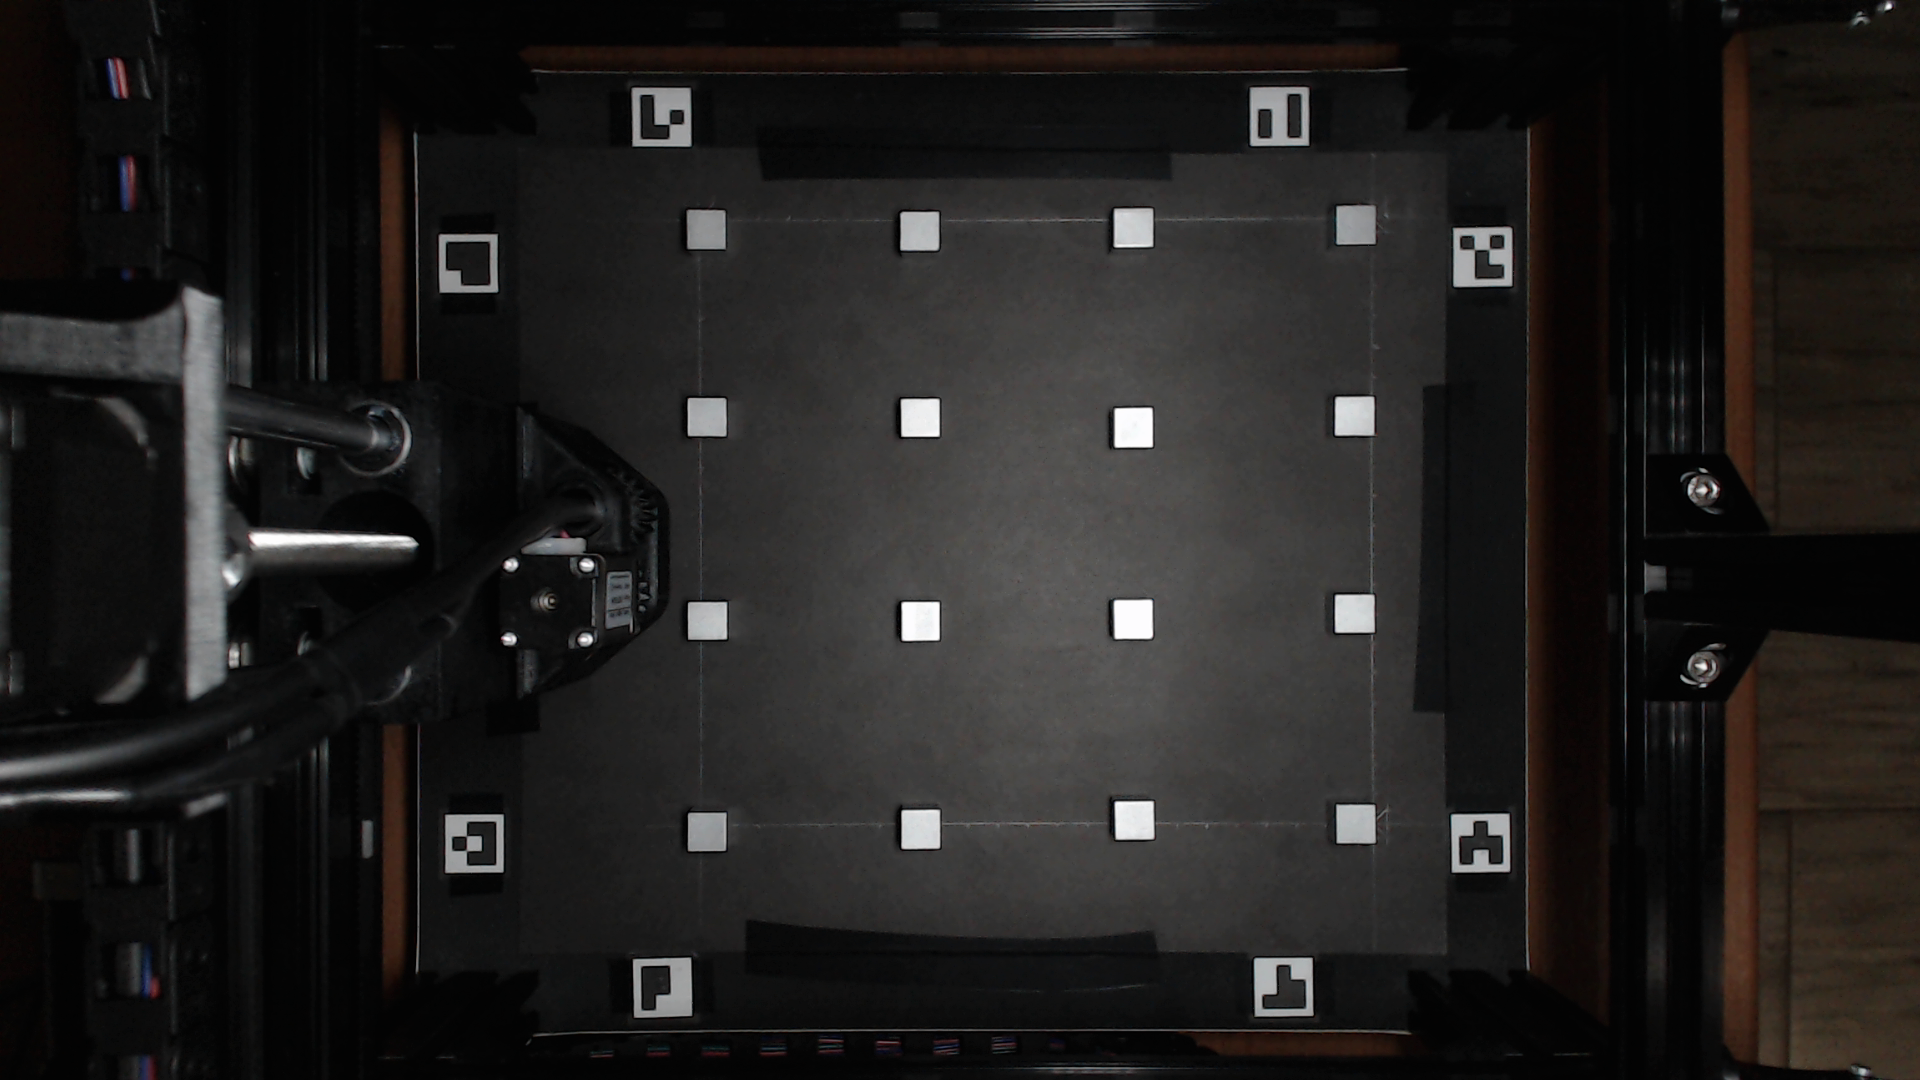
\includegraphics[width=1\linewidth]{figures/qtp6-set1.png}
	\caption{First test set of known cube positions and orientations (0$\degree$) in the robot's workspace for qualification test 6.}
	\label{fig:qtp6-set1}
\end{figure}

\begin{figure}[H]
	\centering
	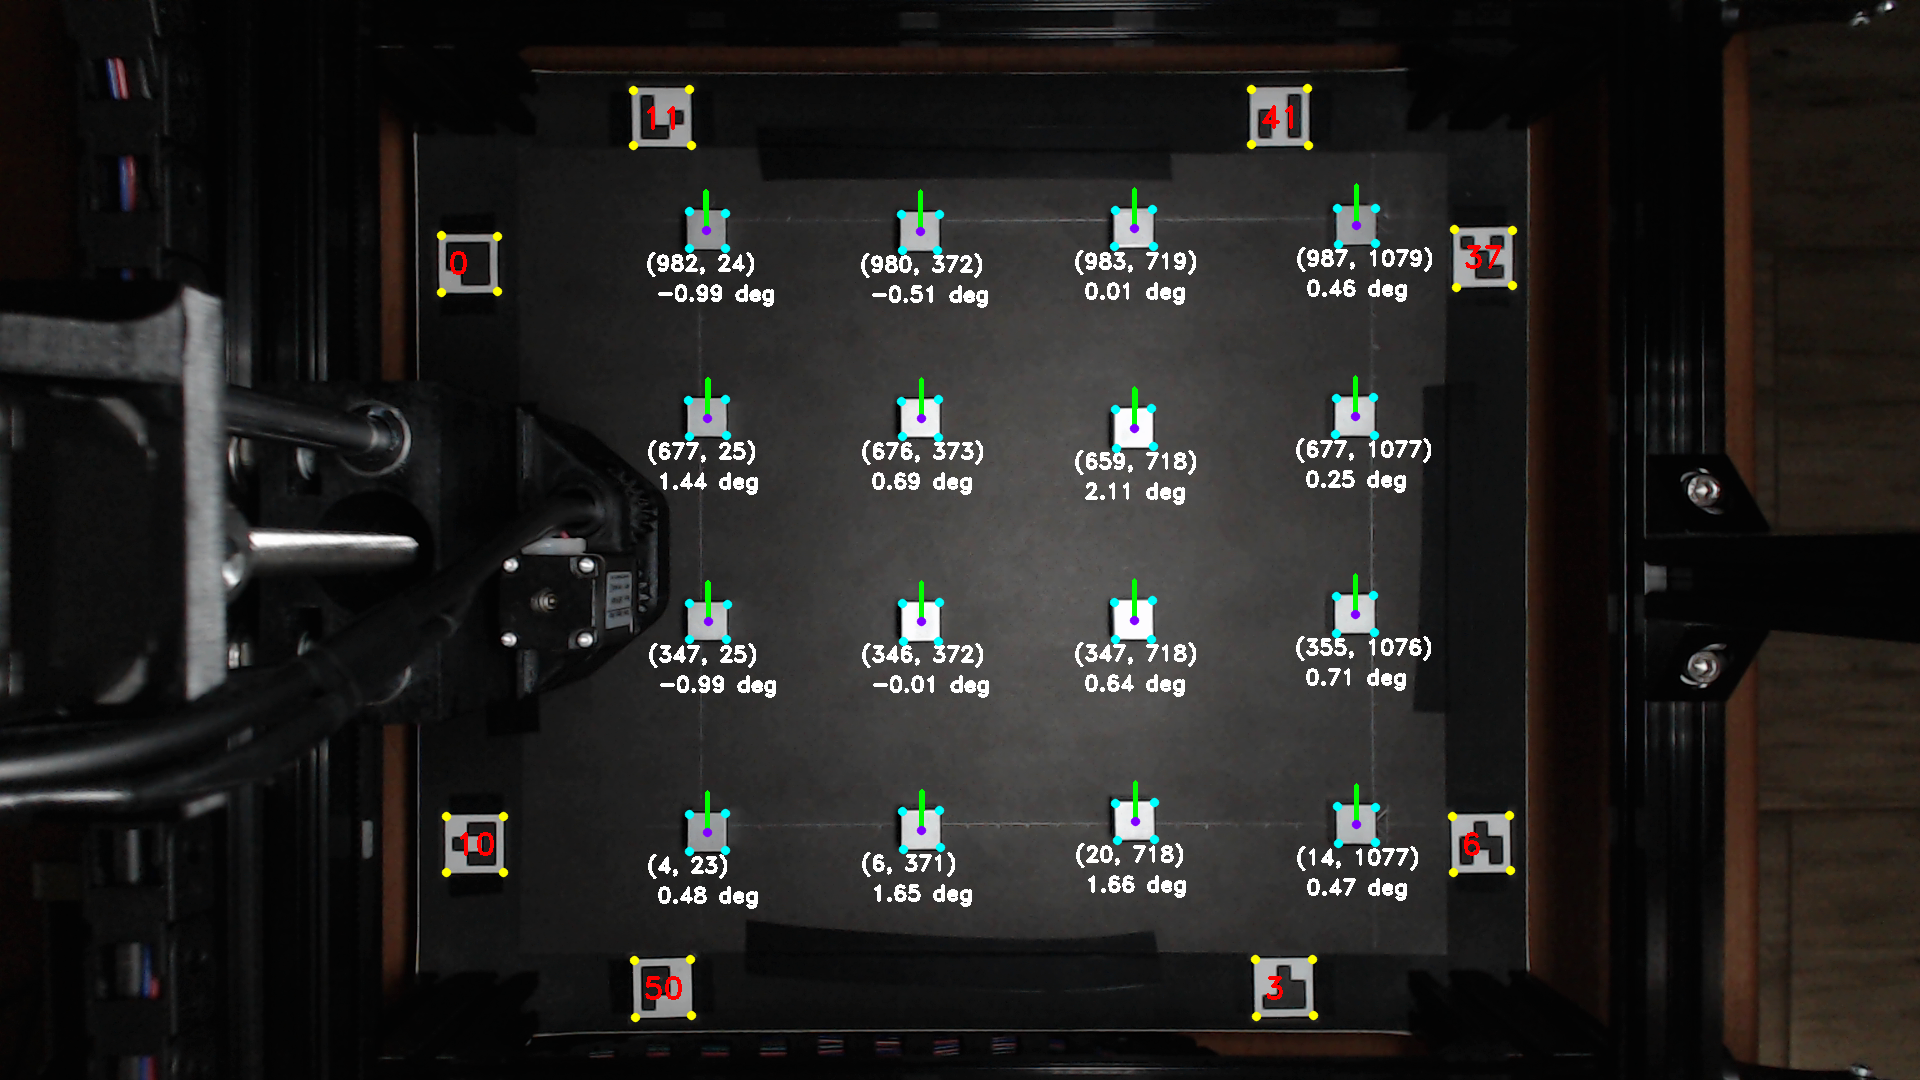
\includegraphics[width=1\linewidth]{figures/qtp6-set1-annotated.png}
	\caption{First test set of cubes after pose estimation by the \textit{Vision System} for qualification test 6.}
	\label{fig:qtp6-set1-annotated}
\end{figure}

\begin{figure}[H]
	\centering
	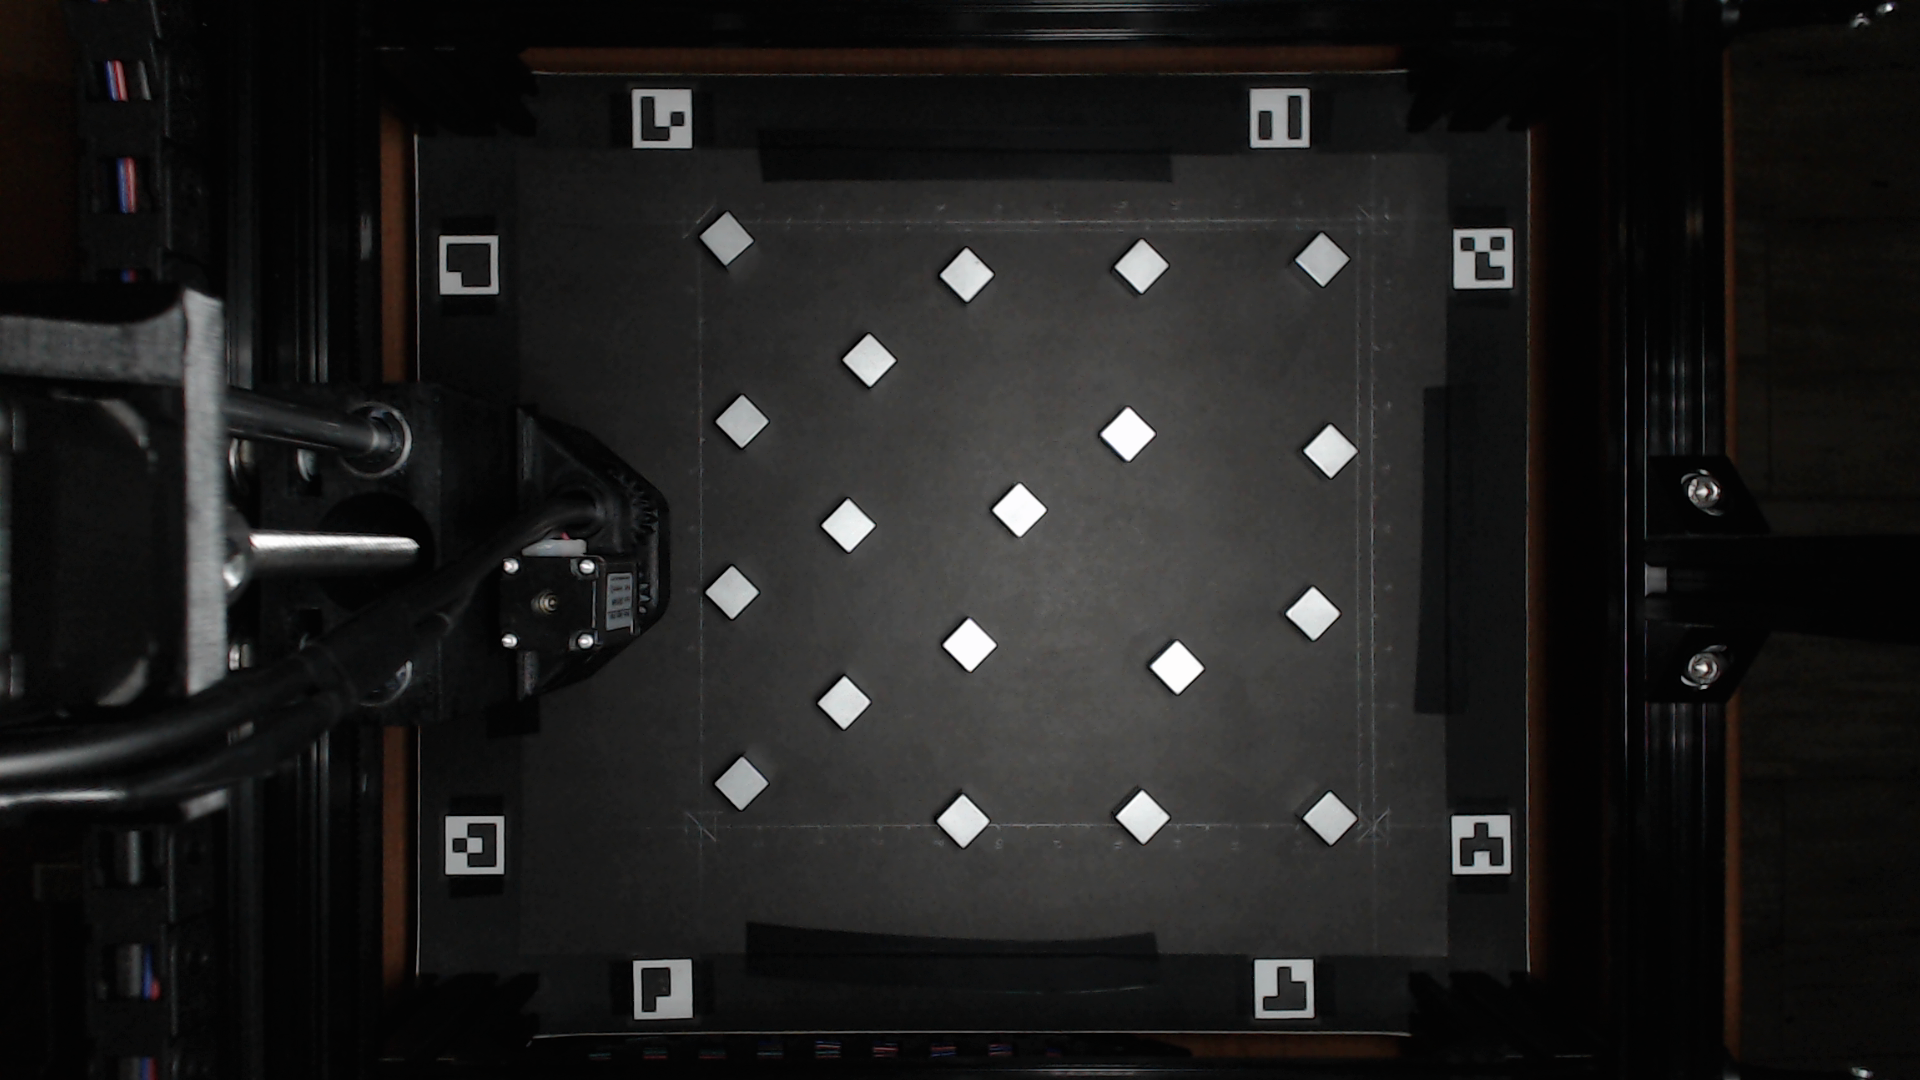
\includegraphics[width=1\linewidth]{figures/qtp6-set2.png}
	\caption{Second test set of known cube positions and orientations (45$\degree$) in the robot's workspace for qualification test 6.}
	\label{fig:qtp6-set2}
\end{figure}

\begin{figure}[H]
	\centering
	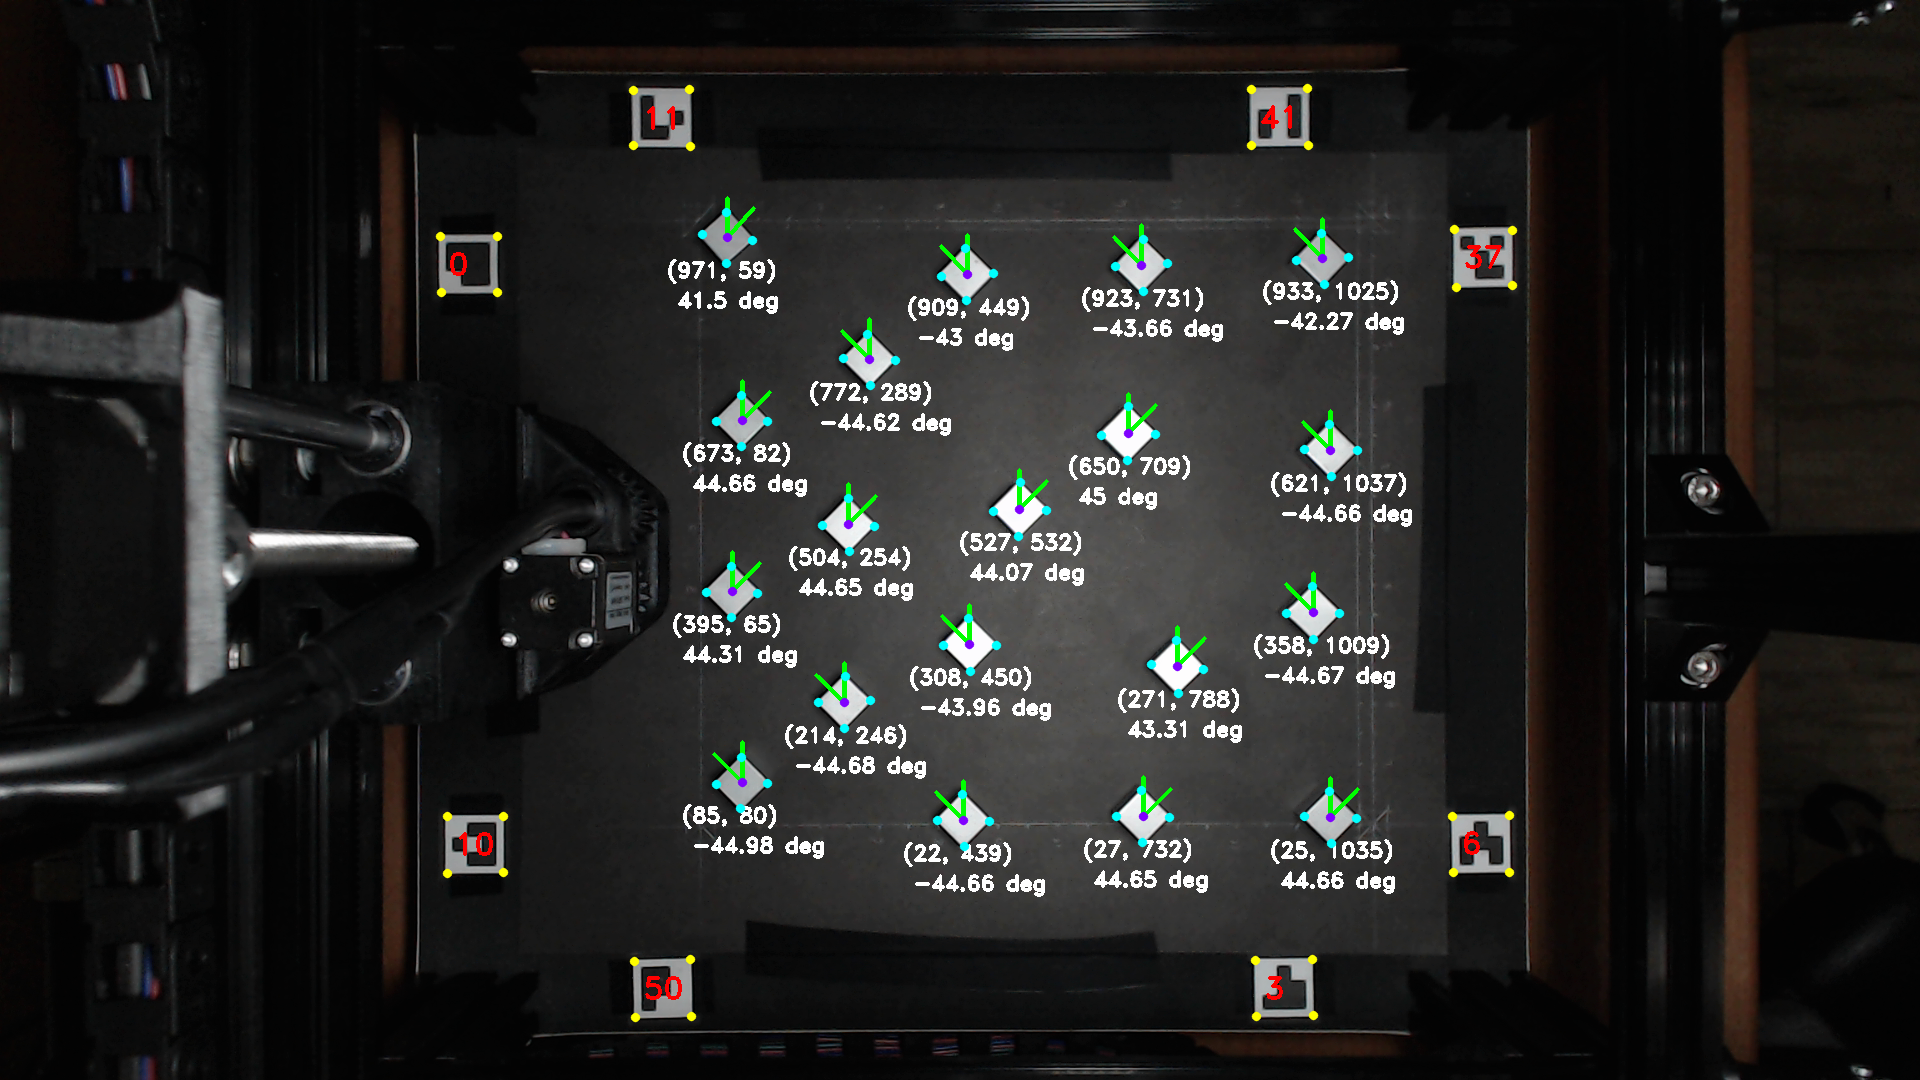
\includegraphics[width=1\linewidth]{figures/qtp6-set2-annotated.png}
	\caption{Second test set of cubes after pose estimation by the \textit{Vision System} for qualification test 6.}
	\label{fig:qtp6-set2-annotated}
\end{figure}

\subsubsecnonumhidden{Qualification Test 7 Results}

\begin{table}[H]
	\renewcommand{\arraystretch}{1.3}
	\centering
	\begin{tabular}{|>{\raggedright}m{1.8cm}|>{\raggedright}m{1.2cm}|>{\raggedright}m{1.2cm}|>{\raggedright}m{1.2cm}|>{\raggedright}m{1.2cm}|>{\raggedright}m{1.2cm}|>{\raggedright\arraybackslash}m{3cm}|}
		\hline
		\multirow{2}{1.8cm}{\textbf{Iteration}} & \multicolumn{5}{|l|}{\textbf{Dropped Cubes Detected?}} & \multirow{2}{3cm}{\textbf{Failure\- Detected (Y/N)?}} \\ \cline{2-6}
		& \textbf{1-5} & \textbf{6-10} & \textbf{11-15} & \textbf{16-20} & \textbf{21-25} & \\ \hline
		1 & Yes & Yes & Yes & Yes & Yes & Yes \\ \hline
		2 & Yes & Yes & Yes & Yes & Yes & Yes \\ \hline
		3 & Yes & Yes & Yes & Yes & Yes & Yes \\ \hline
		4 & Yes & Yes & Yes & Yes & Yes & Yes \\ \hline
		5 & Yes & Yes & Yes & Yes & Yes & Yes \\ \hline
	\end{tabular}
	\caption{\label{tab:techdoc-qtp7}Results of qualification test 7 to assess capability of system to detect dropped cubes and construction failures.}
\end{table}


%% End of File.


